\def\baselinestretch{1}
\chapter{Simulaci\'on}
\def\baselinestretch{1.0}

\section{Introducci\'on}
Para entender mejor la funcionalidad del \'Indice de Disimilaridad, es necesario realizar algunas simulaciones donde se examine �como funciona te\'oricamente por simulaci\'on? y desde ah\'i, explicar mejor esta nueva medida para clasificar series temporales. Como se mencion\'o anteriormente el \'Indice de Disimilaridad considera la distancia entre las series ponderada por una funci\'on  adaptable de afinaci\'on que balancea la proximidad con relaci\'on a los valores y la proximidad con relaci\'on al comportamiento. La contribuci\'on del comportamiento y componentes de valores para el \'Indice de Disimilaridad es comparada con las medidas convencionales.

La idea es sensibilizar esta medida y compararla con las distancias convencionales que fueron definidas anteriormente y ver cuales son sus diferencias.

El objetivo de este cap\'itulo es implementar un algoritmo de clasificaci\'on para series temporales. Se espera que el \'Indice de Disimilaridad al considerar la informaci\'on del comovimiento agrupe las series, que las medidas convencionales no agrupan, es decir, se quiere demostrar que este \'Indice agrupa series temporales con una justificaci\'on mayor que las distancias convencionales.

\section{Simulaci\'on entre series correlacionadas}

Antes de representar y graficar la funcionalidad del \'Indice de Disimilaridad es necesario explicar, cuales son las condiciones de esta simulaci\'on, detallar los modelos que ser\'an analizados con sus respectivas caracter\'isticas.

Los elementos necesarios para esta simulaci\'on es la estructura de correlaci\'on de los errores. Por ejemplo, considere la siguiente estructura de correlaci\'on:
%\begin{eqnarray}
%x&=&y\label{prime}\\
%x^2&=&xy\nonumber\\
%x^2-y^2&=&xy-y^2\nonumber\\
%(x+y)(x-y)&=&y(x-y)\nonumber\\
%x+y&=&y\nonumber\\
%2y&=&y\quad \mbox{por (\ref{prime})}\nonumber\\
%2&=&1\nonumber
%\end{eqnarray}

\begin{eqnarray}
\mathbb Cov(\epsilon_{c}(t),\epsilon_{b}(s)) = \left\{
\begin{array}{cl}
\rho\tau\sigma&\mbox{si } t=s\\
0&\mbox{eoc }
\end{array}\right..
\end{eqnarray}

Donde $\epsilon_{c}(t)$ y $\epsilon_{b}(t)$, son errores correlacionados con media 0 y varianza $\tau^{2}$, $\sigma^{2}$, respectivamente.\\
Seguidamente, esta estructura se aplicar\'a para 7 modelos AR(1), cada uno con errores $\{\epsilon_{i},i=1,\ldots,7\}$ aleatorios independientes id\'enticamente distribu\'idos normal con media 0 y varianza $\sigma^{2}$.

Para verificar las bondades del \'Indice de Disimilaridad antes mencionados, intencionalmente se simularan errores $\epsilon_2(t)$ y $\epsilon_3(t)$  que estar\'an correlacionados con $\epsilon_1(t)$. Entonces, dependiendo de que valor se le de a cada correlaci\'on $\rho_1$ y $\rho_2$ es cuan correlacionados estar\'an los errores. Se esperar\'ia que el \'Indice de Disimilaridad agrupara primero las series con los errores que fueron intencionalmente correlacionados.

Ahora, considere la siguiente estructura de correlaci\'on:
\begin{eqnarray*}
corr(\epsilon_{1}(t),\epsilon_{2}(s)) &=&\rho_1,\mbox{ $t=s$,}\\
corr(\epsilon_{1}(t),\epsilon_{3}(s)) &=& \rho_2, \mbox{ $t=s$.}\\
\end{eqnarray*}

Los valores de $\rho_{1}$ y $\rho_{2}$, ayudaran a diferenciar los otros 4 modelos en los cuales sus errores ser\'an variables independientes normales con media 0 y varianza 1.

Otra forma de considerar estos errores correlacionados, es a trav\'es de una matriz de correlaci\'on para el vector $\b{v}=(\epsilon_{1},\epsilon_{2},\epsilon_{3})^{t}$, donde cada $\epsilon_{i},i=1,2,3$ tiene varianza $\sigma^{2}$, $\tau^{2}$ y $\eta^{2}$, respectivamente. Entonces, el proceso es simulado con la estructura para la covarianza $\Sigma$.

\begin{displaymath}
\mathbf{\Sigma} =
\left( \begin{array}{ccc}
\sigma^{2} & \rho_{1}\tau\sigma & \rho_{2}\sigma\eta \\
\rho_{1}\tau\sigma & \tau^{2} & \rho\tau\eta \\
\rho_{2}\sigma\eta & \rho\tau\eta & \eta^{2}
\end{array} \right),
\end{displaymath}

y como consecuencia la matriz de correlaci\'on del vector de errores $\b{v}$ es:

\begin{displaymath}
\mathbf{\mathbb Corr(\b{v})} =
\left( \begin{array}{ccc}
1 & \rho_{1} & \rho_{2} \\
\rho_{1} & 1 & \rho \\
\rho_{2} & \rho & 1
\end{array} \right).
\end{displaymath}

Luego, en estructura de correlaci\'on se incorpora otro elemento que ayudar\'a entender mejor esta nueva medida. Se definen 7 modelos AR(1), los cuales 3 de ellos tendr\'an una caracter\'istica en com\'un, difiriendo en el grado de interdependencia.

Ahora, ya creados los errores con la estructura de correlaci\'on antes mencionada para $\epsilon_{2}$ y $\epsilon_{3}$ correlacionadas con $\epsilon_{1}$, se incorporan en los modelos $Y_t$ y $W_t$.\\
Finalmente, se construyen los siguientes modelos AR(1):
\begin{eqnarray*}
X_t&=&\phi_{1}X_{t-1}+\epsilon_1(t)\\
Y_t&=&\phi_{2}Y_{t-1}+\epsilon_2(t)\\
W_t&=&\phi_{3}W_{t-1}+\epsilon_3(t)\\
V_t&=&\phi_{4}V_{t-1}+\epsilon_4(t)\\
T_t&=&\phi_{5}T_{t-1}+\epsilon_5(t)\\
U_t&=&\phi_{6}U_{t-1}+\epsilon_6(t)\\
Z_t&=&\phi_{7}Z_{t-1}+\epsilon_7(t)
\end{eqnarray*}
En todos los casos $|\phi_{i}|<1$ para $i=1,2,\ldots,7$ para estar en presencia de series estacionarias. En las simulaciones los par\'ametros fueron $\phi_{1}=-0.5$; $\phi_{2}=0.3$; $\phi_{3}=-0.8$; $\phi_{4}=0.7$; $\phi_{5}=0.1$; $\phi_{6}=-0.9$ y $\phi_{7}=0.2$, $\rho_1=0.9$ y $\rho_2=0.7,n=200$. Donde $\{\epsilon_{i}\}$ con $i=4,5,6,7$ son variables aleatorias independientes normal con media 0 y varianza 1.

\begin{figure}[!htp]
\centering
\fbox{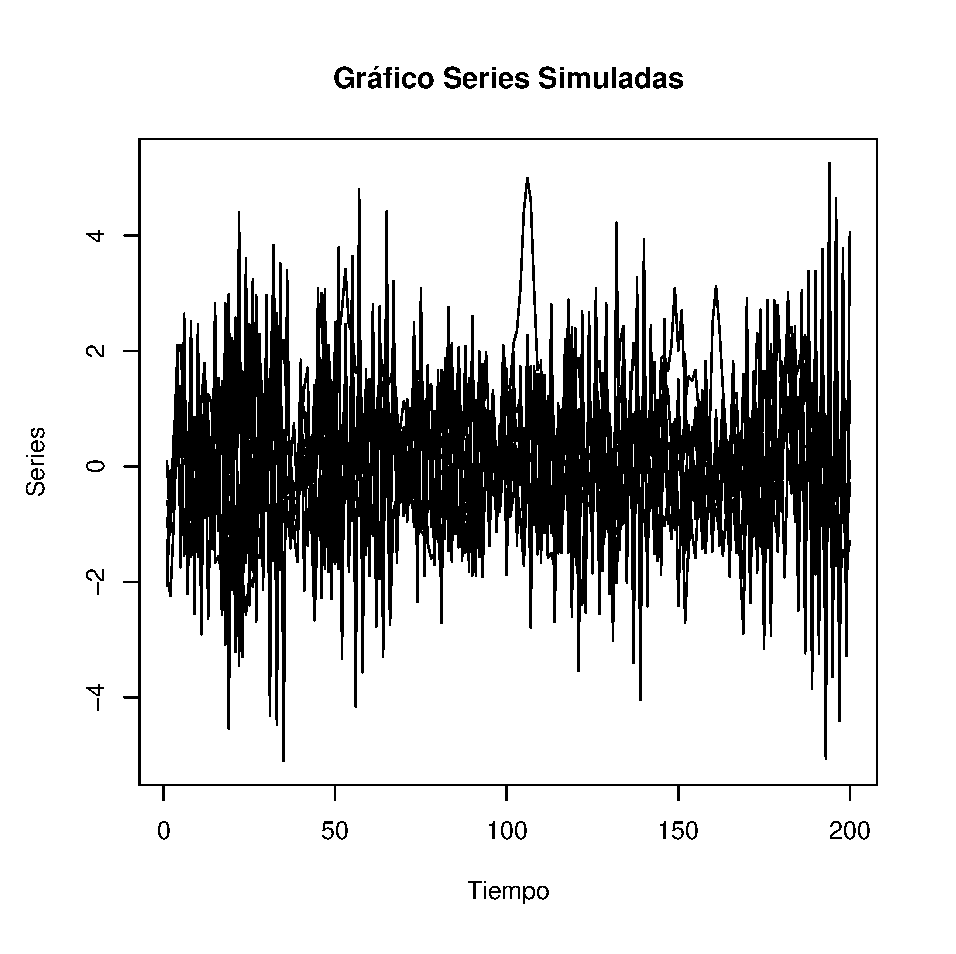
\includegraphics[height=4cm, width=6cm]{s_simu.eps}}
\caption{Series simuladas}
\label{caja}
\end{figure}

En este gr\'afico se puede observar un conjunto de series estacionarias.\\

\begin{figure}[!htp]
\centering
\fbox{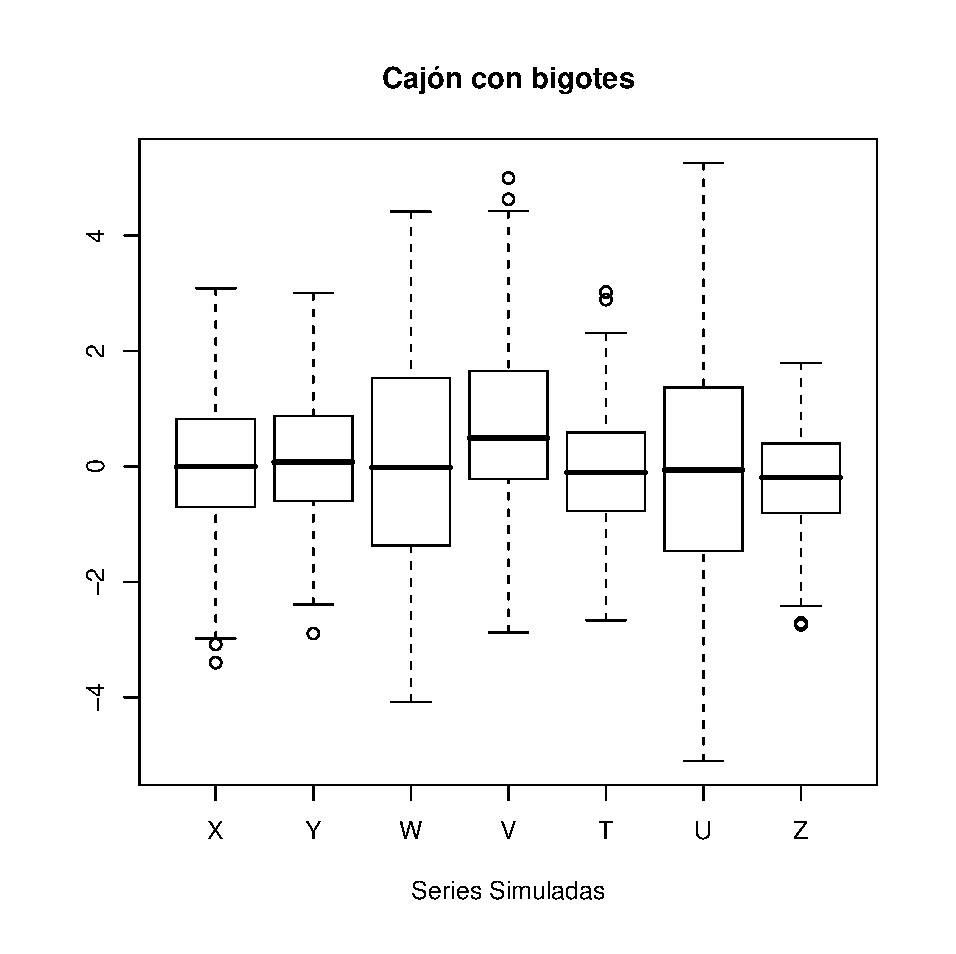
\includegraphics[height=4cm, width=6cm]{cajon_simu.eps}}
\caption{Series simuladas}
\label{caja}
\end{figure}

\newpage
Adem\'as, si aplicamos el algoritmo de clasificaci\'on con las distancias convencionales, se pueden obtener los siguientes resultados.

\begin{figure}[!htp]
\centering
\fbox{ 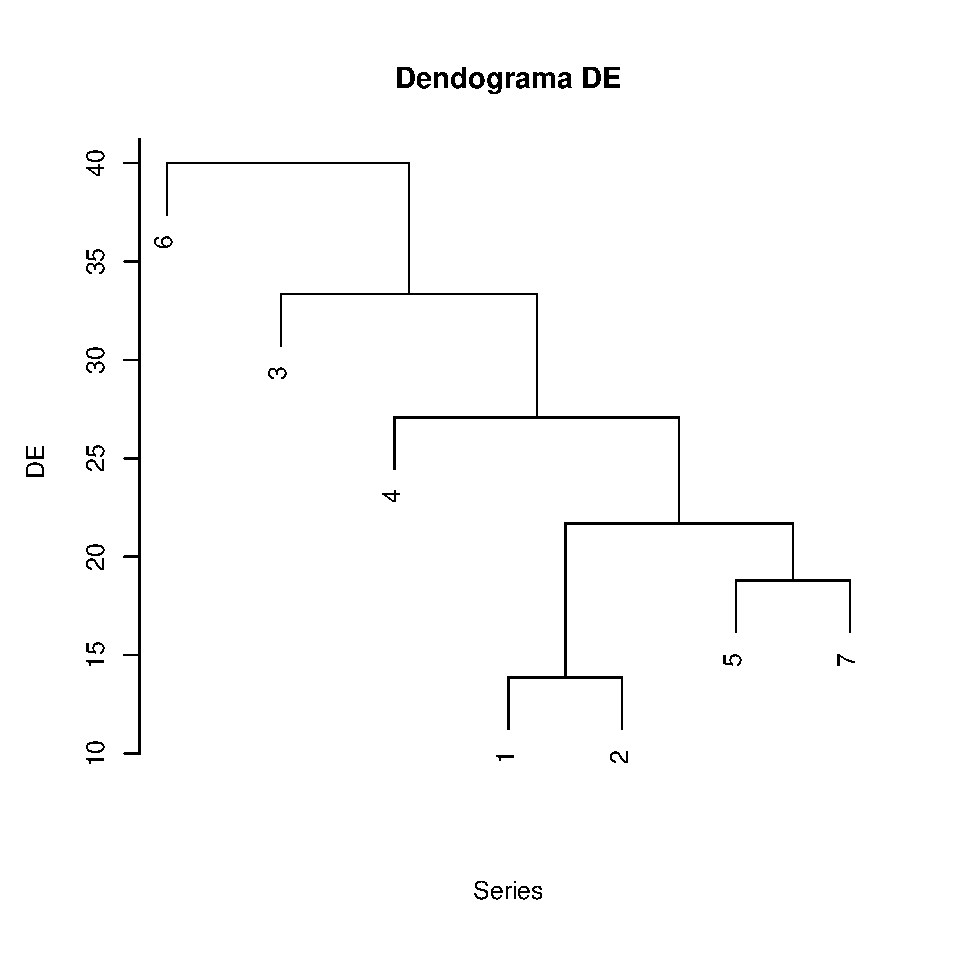
\includegraphics[height=4cm, width=4cm]{de.eps}
       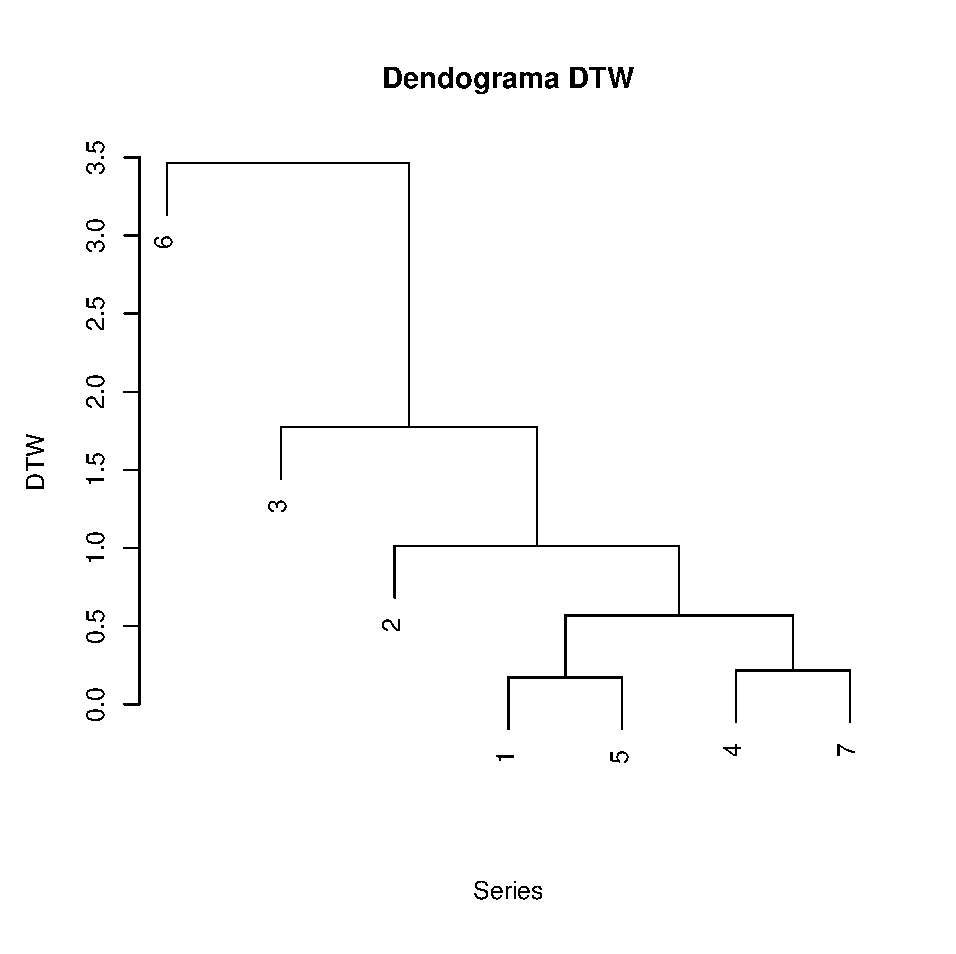
\includegraphics[height=4cm, width=4cm]{dtw.eps}
       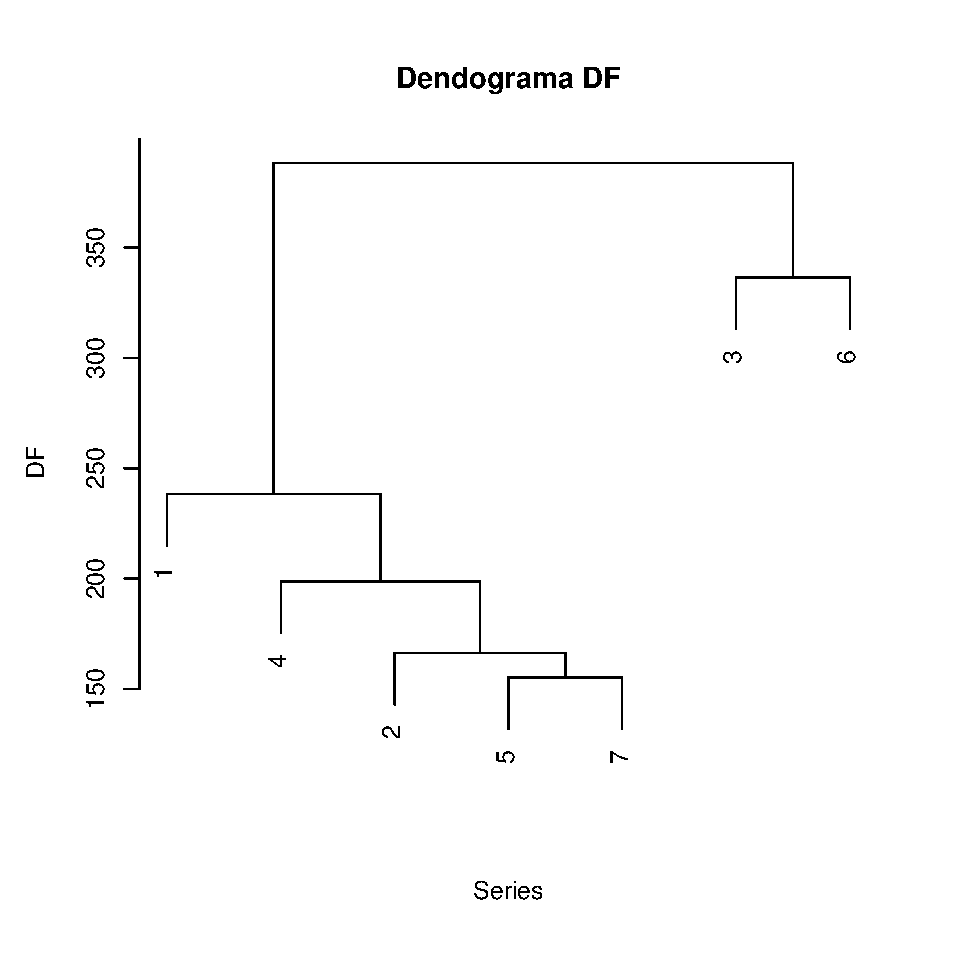
\includegraphics[height=4cm, width=4cm]{df.eps}}
\caption{Dendogramas.}
\label{caja}
\end{figure}

En base a la informaci\'on de las distancias convencionales y con el algoritmo de clasificaci\'on utilizando el m\'etodo jer\'arquico, del vecino m\'as cercano, se puede decir que la distancia euclidiana agrupa 2 de las 3 series correlacionadas, en cambio las distancias de Frech\'et y DTW no agrupan ninguna de las series con errores correlacionados.

\subsection{Gr\'aficos Camino Distorsionado}

Una caracter\'istica que tiene la distancia DTW, es gr\'aficar la opci\'on de camino distorsionado entre las series, a continuaci\'on se presentar\'an algunos gr\'aficos con distintas combinaciones entre las distintas series y analizar la similitud entre las series.

\begin{figure}[!htp]
       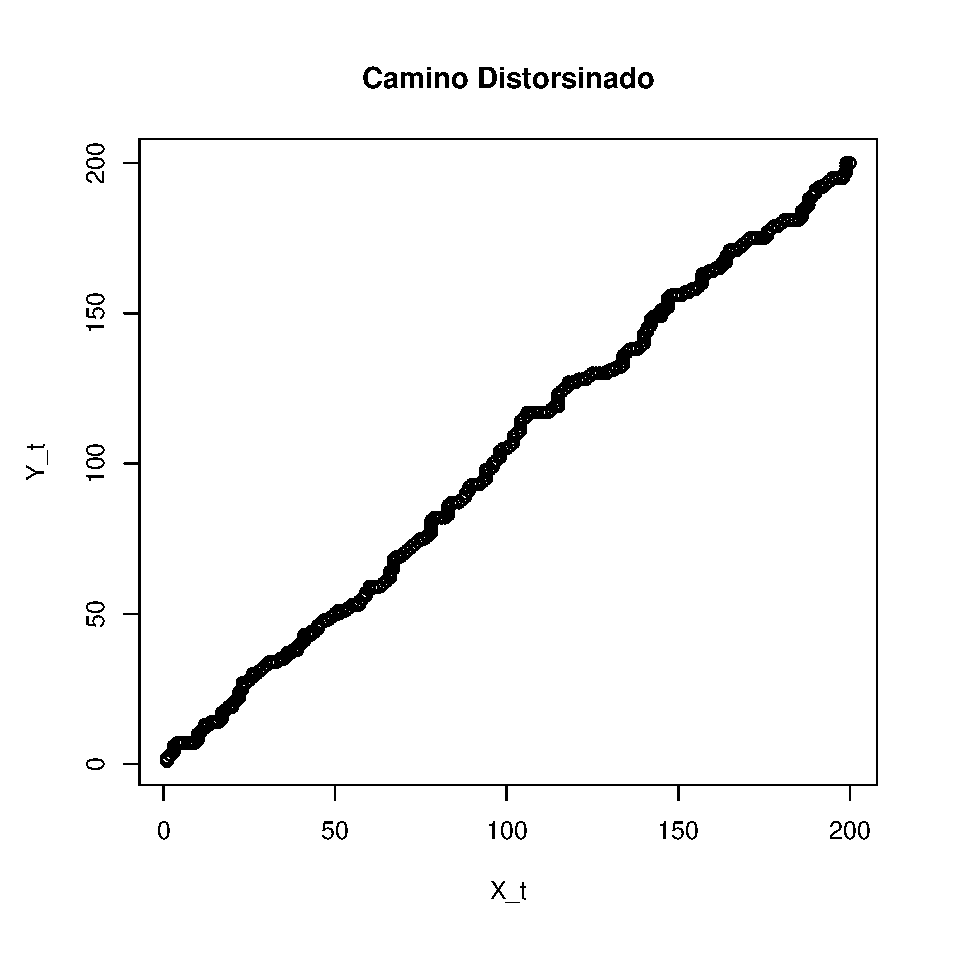
\includegraphics[height=4cm, width=4cm]{cam_dist_xy.eps}
       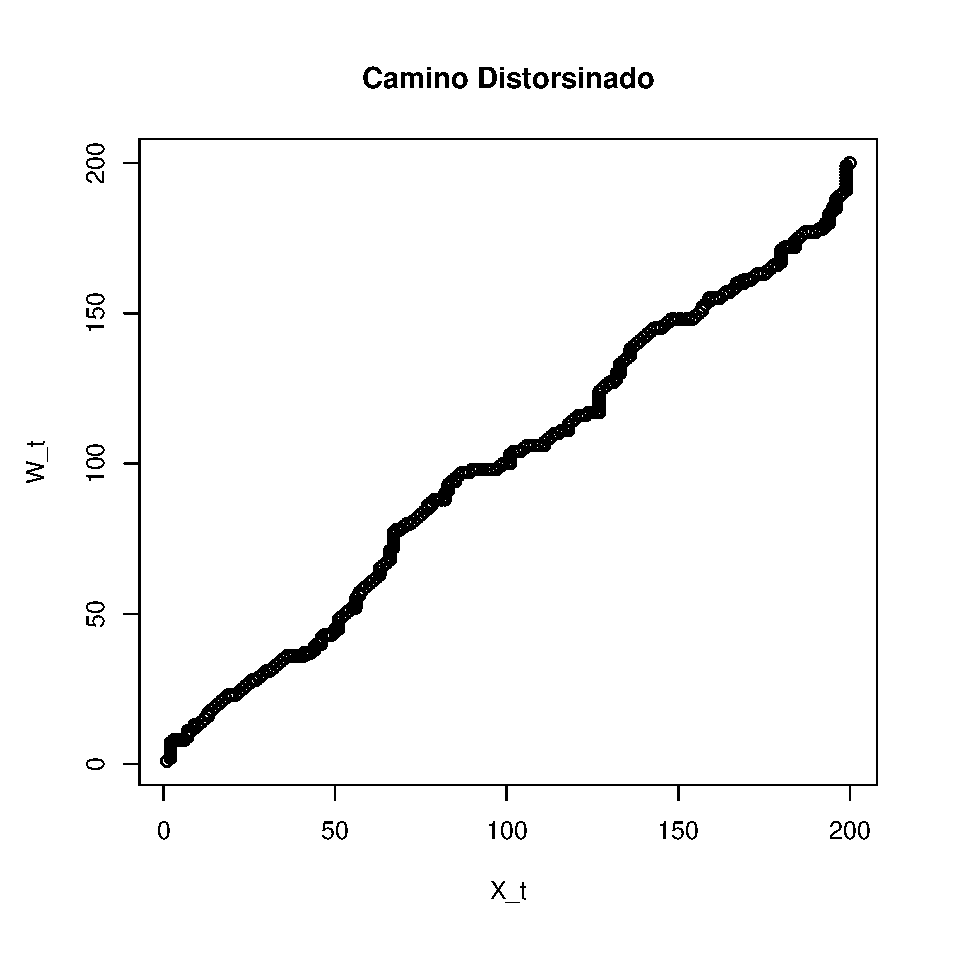
\includegraphics[height=4cm, width=4cm]{cam_dist_xw.eps}
       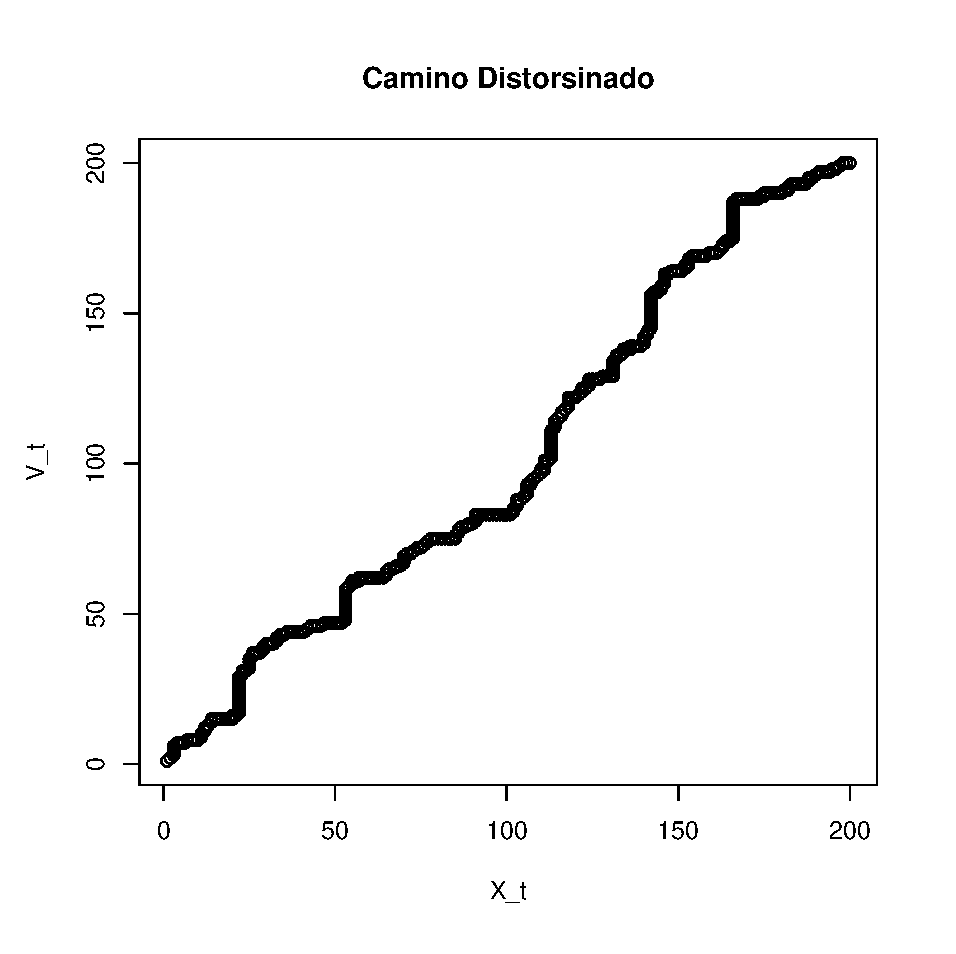
\includegraphics[height=4cm, width=4cm]{cam_dist_xv.eps}
       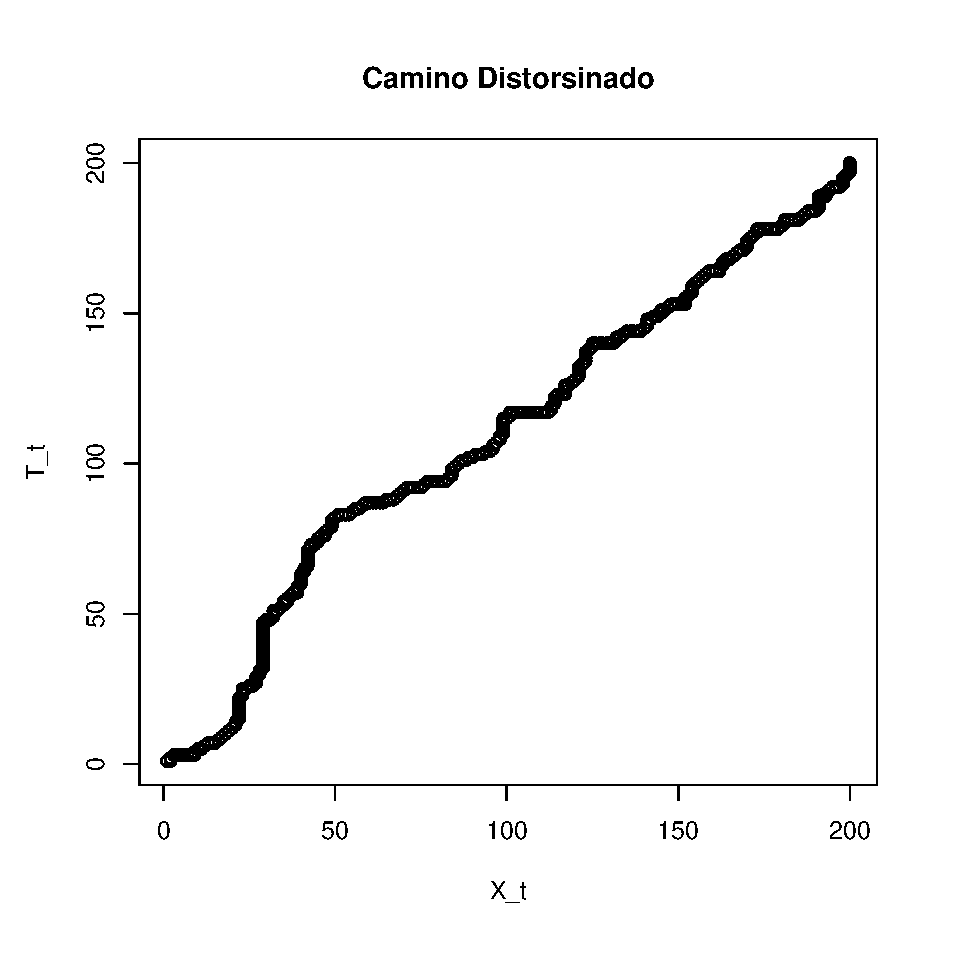
\includegraphics[height=4cm, width=4cm]{cam_dist_xt.eps}
       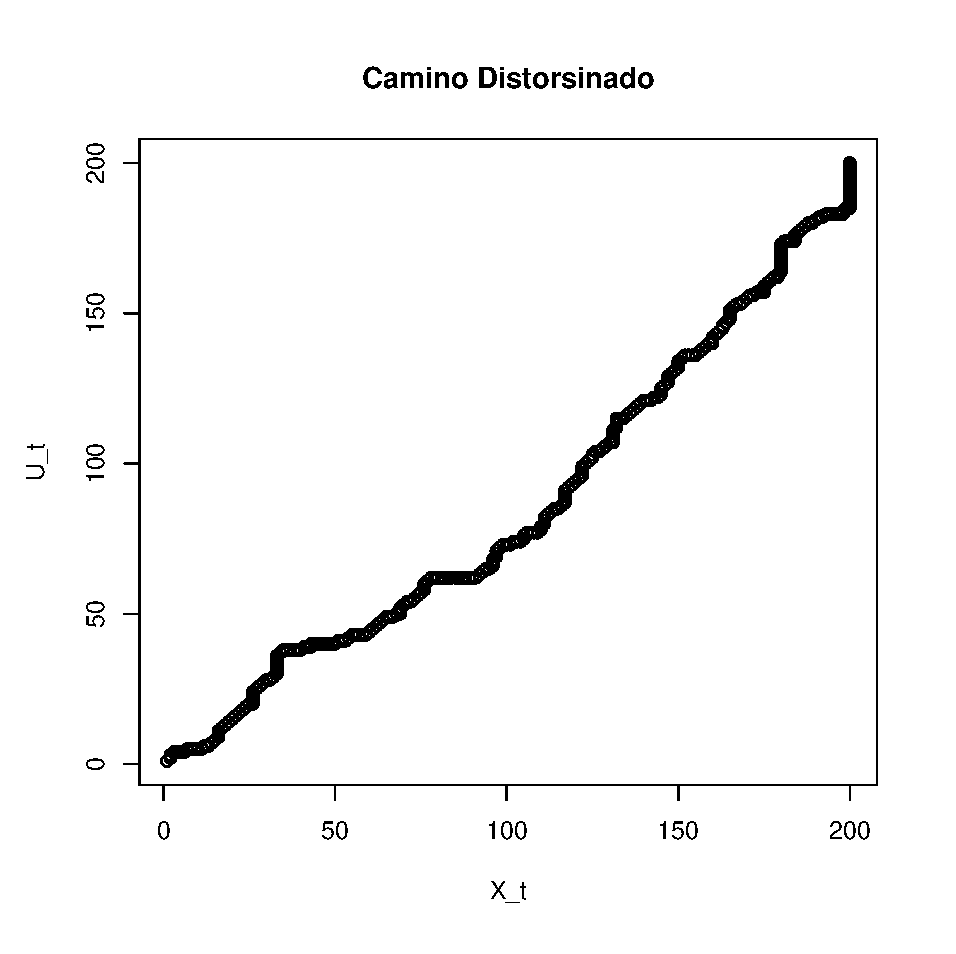
\includegraphics[height=4cm, width=4cm]{cam_dist_xu.eps}
       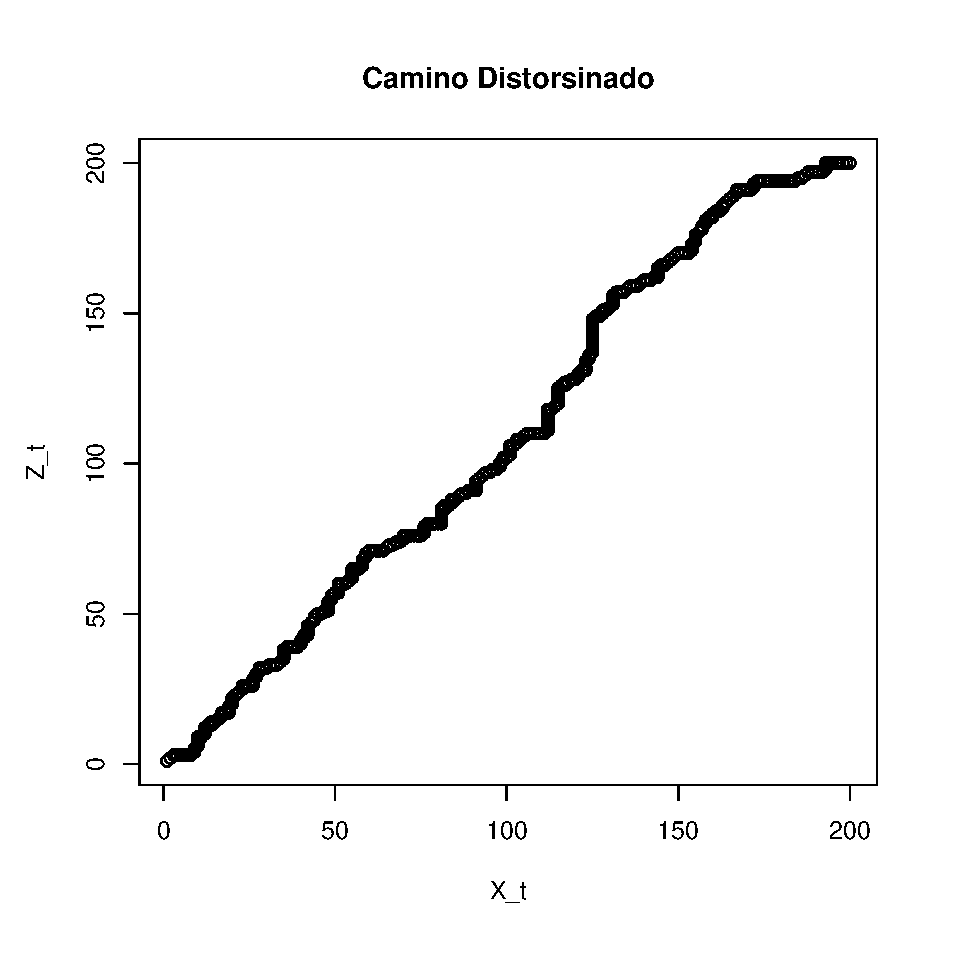
\includegraphics[height=4cm, width=4cm]{cam_dist_xz.eps}
\caption{Camino Distorsionado.}
\label{caja}
\end{figure}

Estos gr\'aficos nos dan una idea de como interactuan las series, se puede apreciar un grado de similitud entre las series, ya que, los puntos del camino distorsionado presentan una recta.\\

Por otra parte, si se aplica el algoritmo de clasificaci\'on con el \'Indice de Disimilaridad Adaptativo con $h=1,2,3$ y $k=1,2,3,4$ se puede observar los siguientes resultados.

\subsection{\'Indice de Disimilaridad Adaptativo con Distancia Euclidiana}

En base a la simulaci\'on y el c\'alculo de las matrices de distancia con esta nueva medida de clasificaci\'on se puede apreciar los siguientes resultados.

El \'Indice con $h=1$ agrupa las series $X_t$, $Y_t$ y $W_t$, como era de esperar, agrupa primero $X_t$ con $Y_t$, ya que sus errores tienen un grado m\'as alto de correlaci\'on, luego incorpora la series $W_t$. A continuaci\'on se presenta el algoritmo de clasificaci\'on para series temporales con $h=2,3$. Se puede observar que para $h=2$, el \'Indice de Disimilaridad mantiene los grupos, que est\'an correlacionados. Con $h=3$, el \'Indice de Disimilaridad mantiene los grupos establecidos.

\begin{figure}[!htp]
       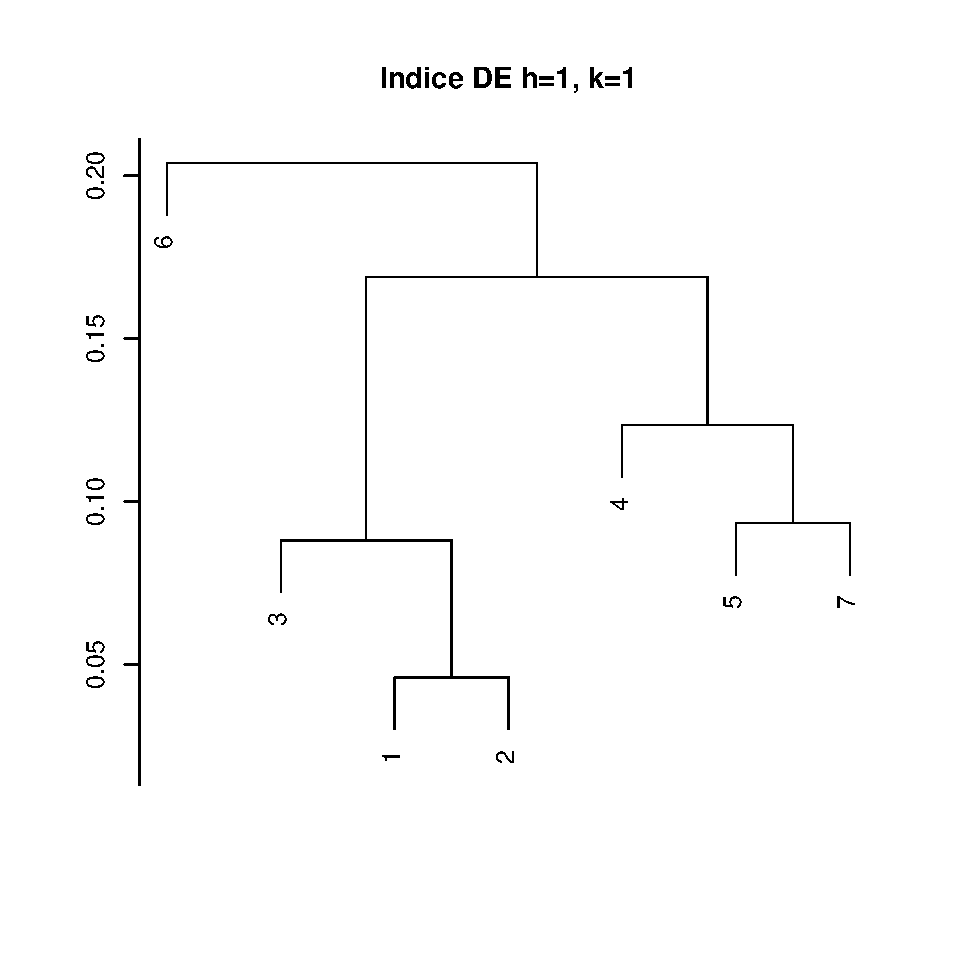
\includegraphics[height=4cm, width=4cm]{d111.eps}
       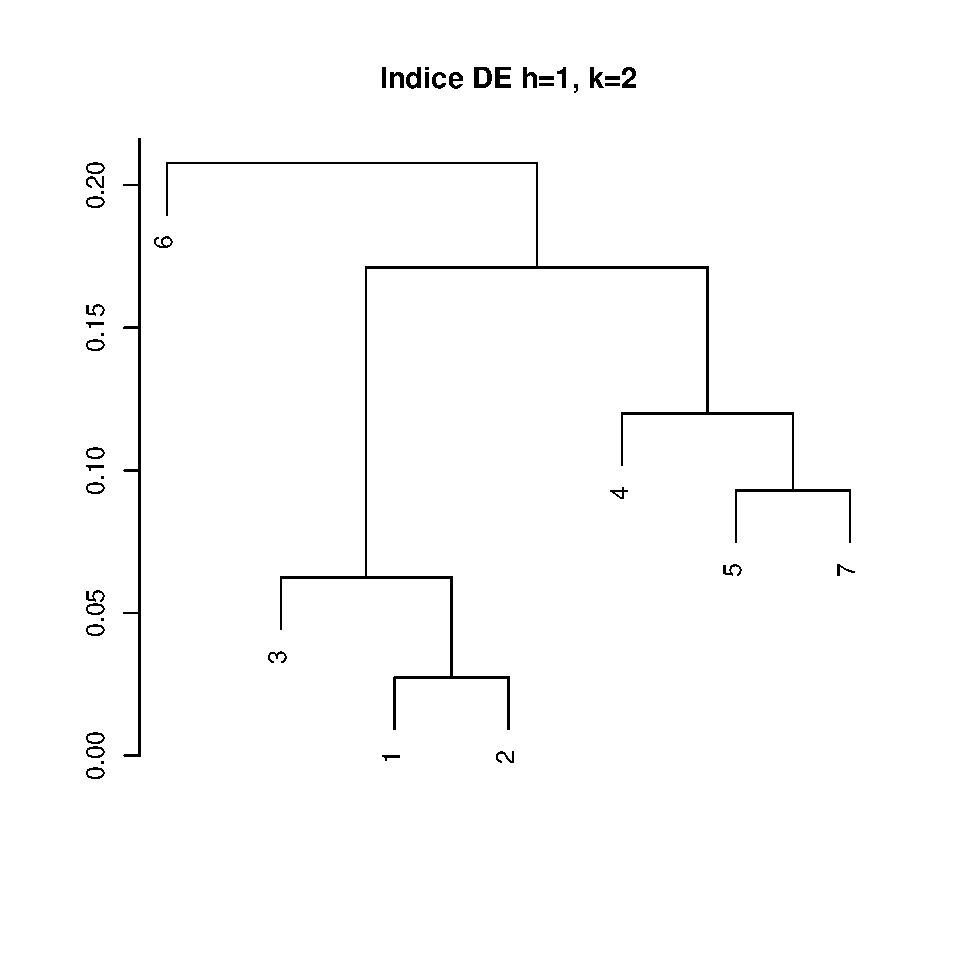
\includegraphics[height=4cm, width=4cm]{d112.eps}
       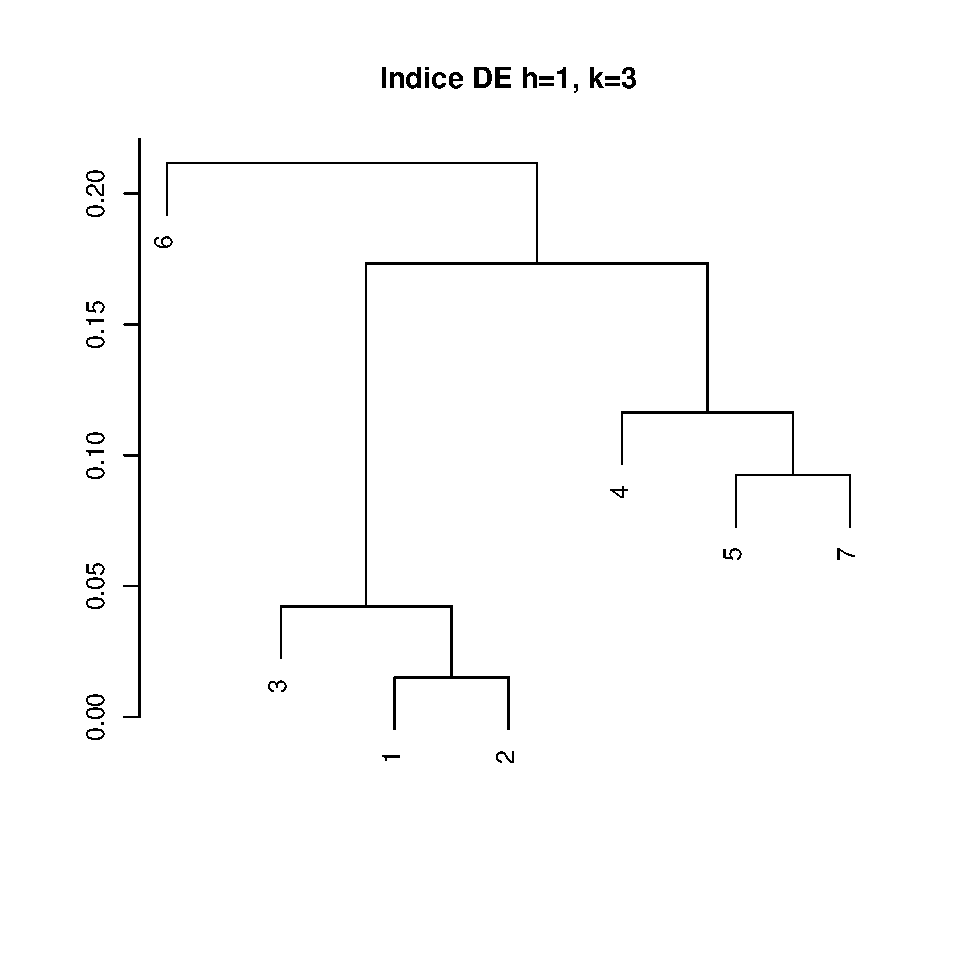
\includegraphics[height=4cm, width=4cm]{d113.eps}
       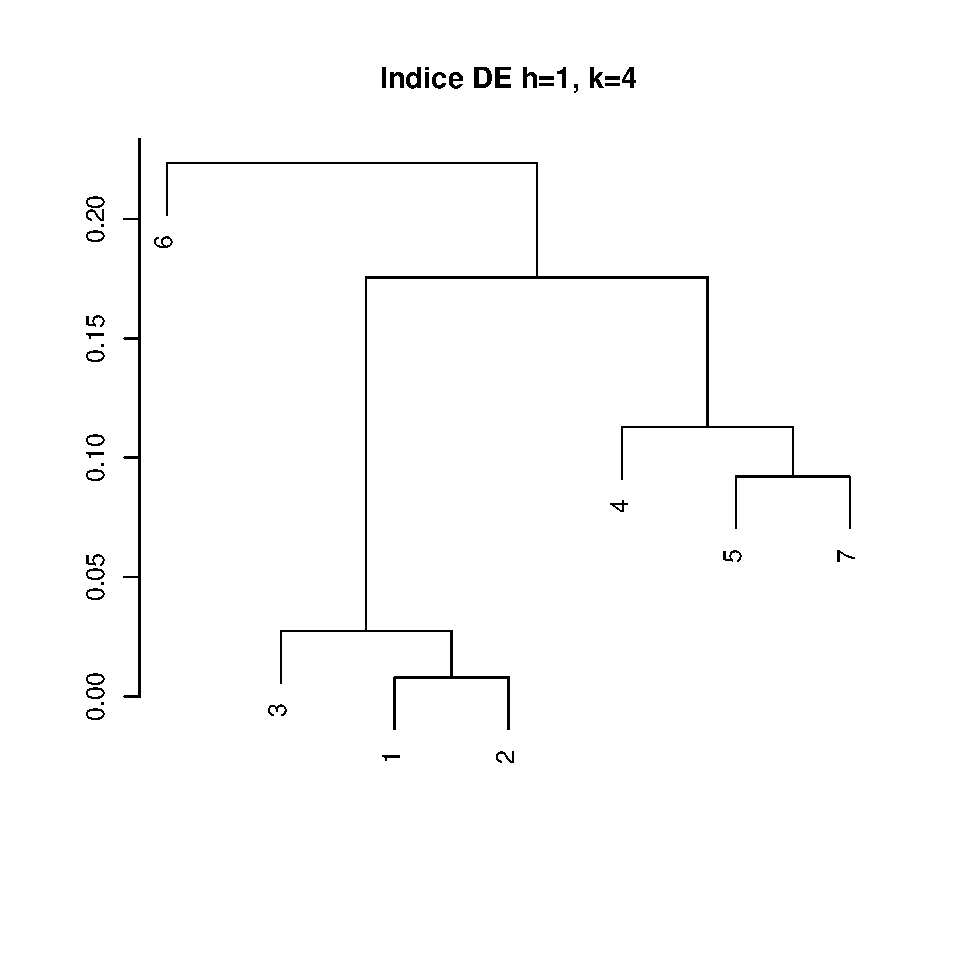
\includegraphics[height=4cm, width=4cm]{d114.eps}
\caption{Dendogramas \'Indice con $\delta_{E}$ con $h=1$, $k=1,2,3,4.$}
\label{caja}
\end{figure}


\begin{figure}[!htp]
       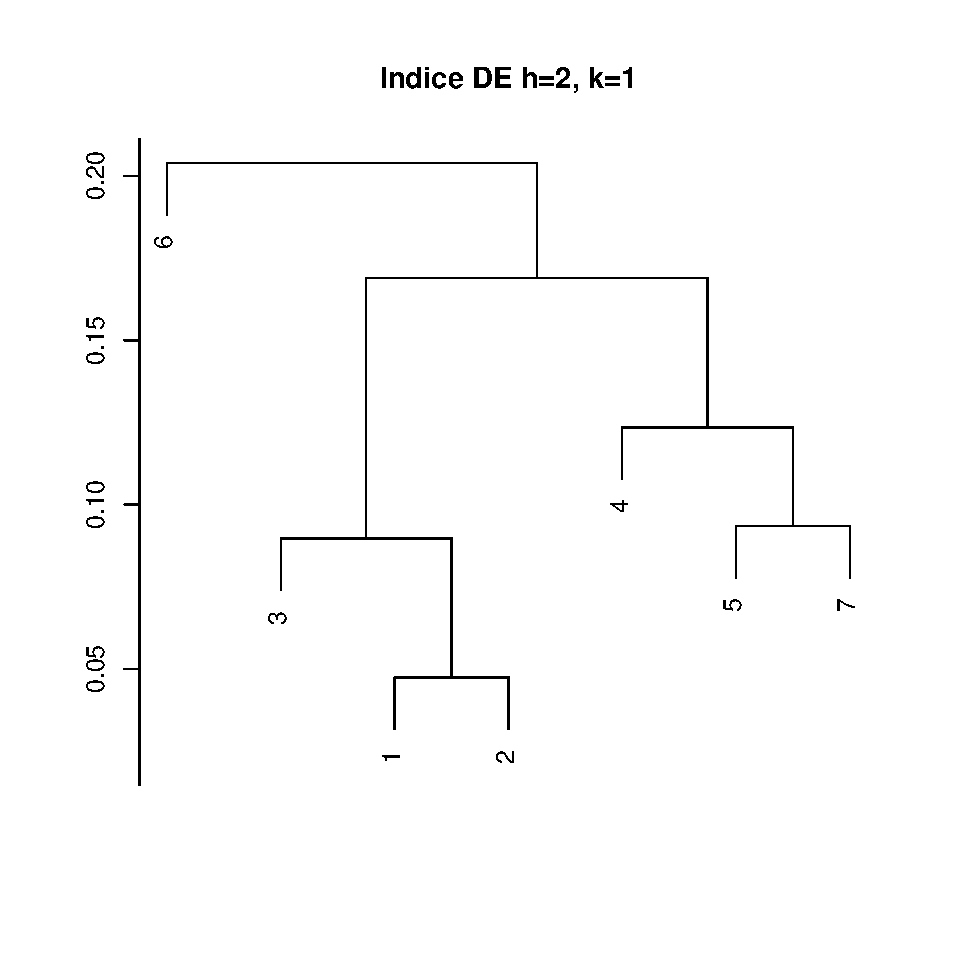
\includegraphics[height=4cm, width=4cm]{d121.eps}
       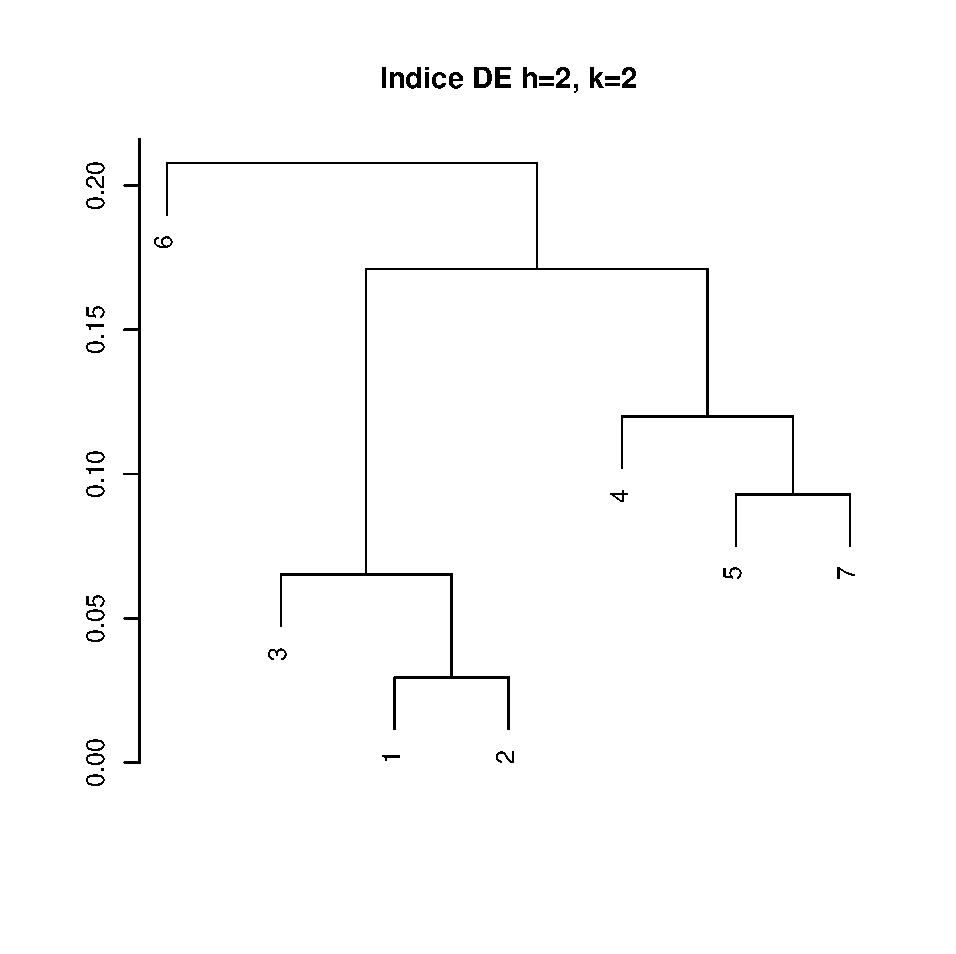
\includegraphics[height=4cm, width=4cm]{d122.eps}
       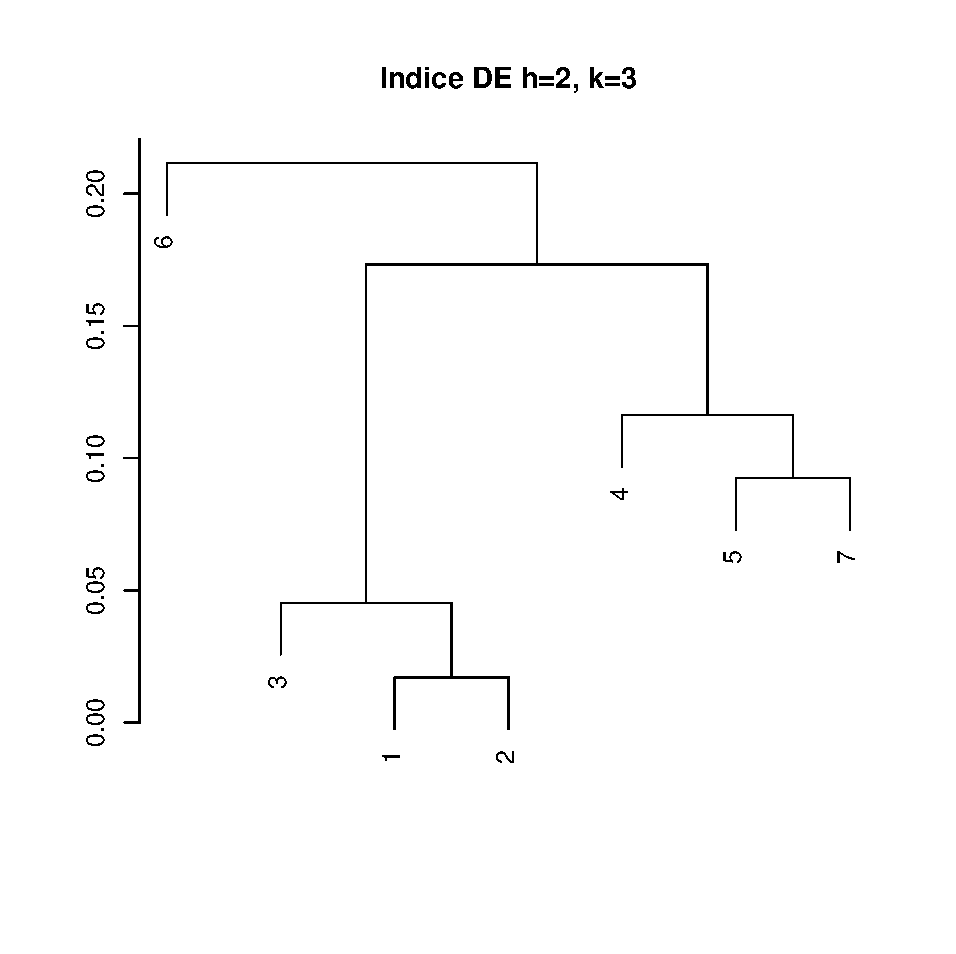
\includegraphics[height=4cm, width=4cm]{d123.eps}
       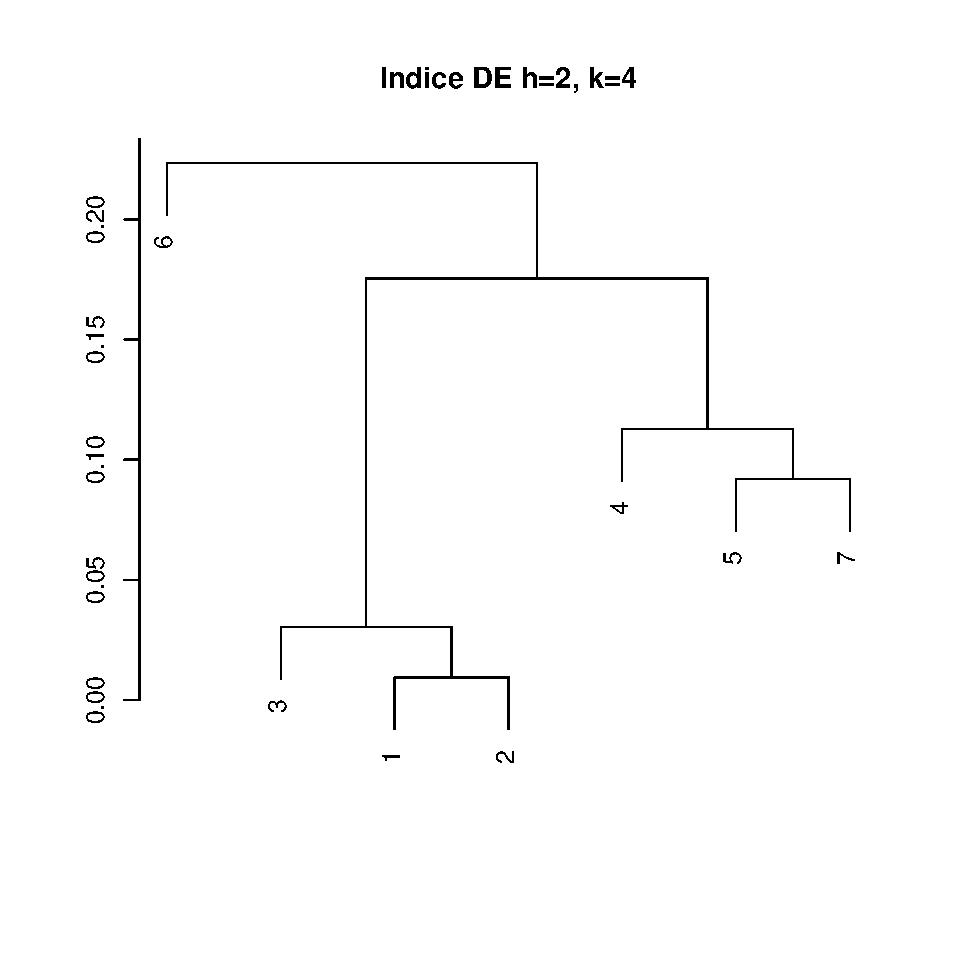
\includegraphics[height=4cm, width=4cm]{d124.eps}
\caption{Dendogramas \'Indice con $\delta_{E}$ con $h=2$, $k=1,2,3,4.$}
\label{caja}
\end{figure}


\begin{figure}[!htp]
       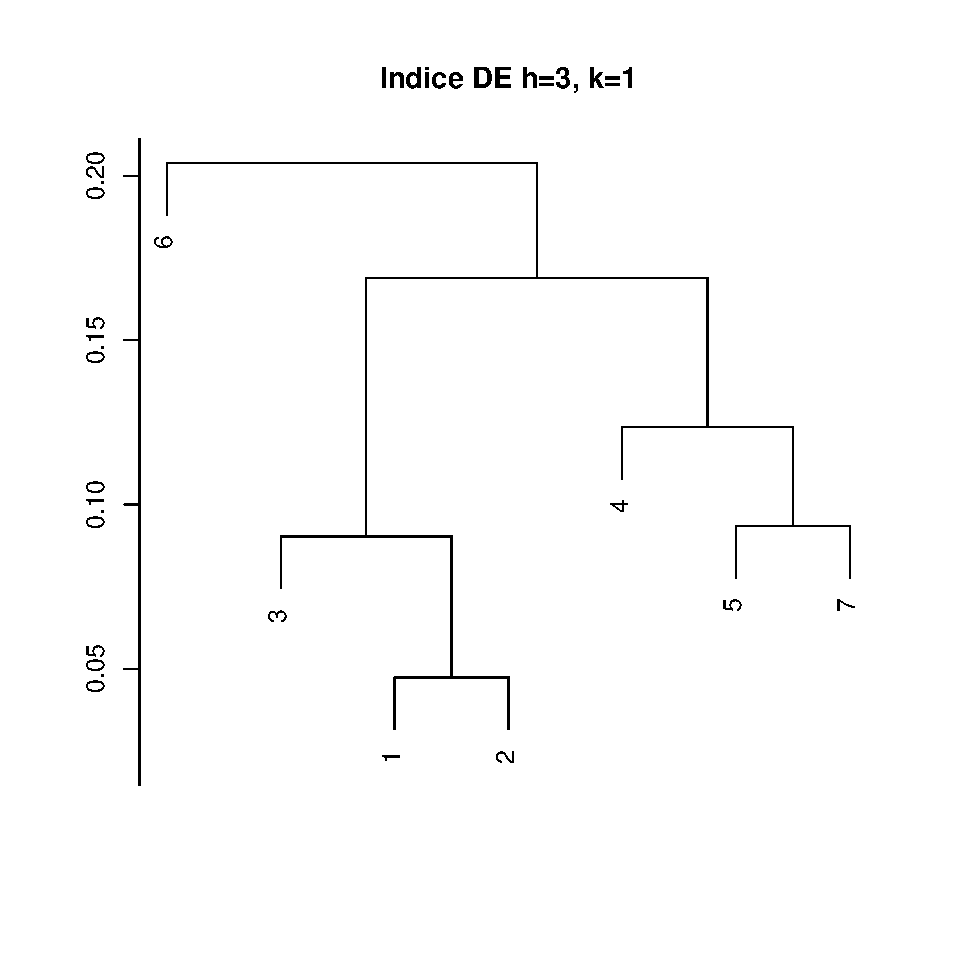
\includegraphics[height=4cm, width=4cm]{d131.eps}
       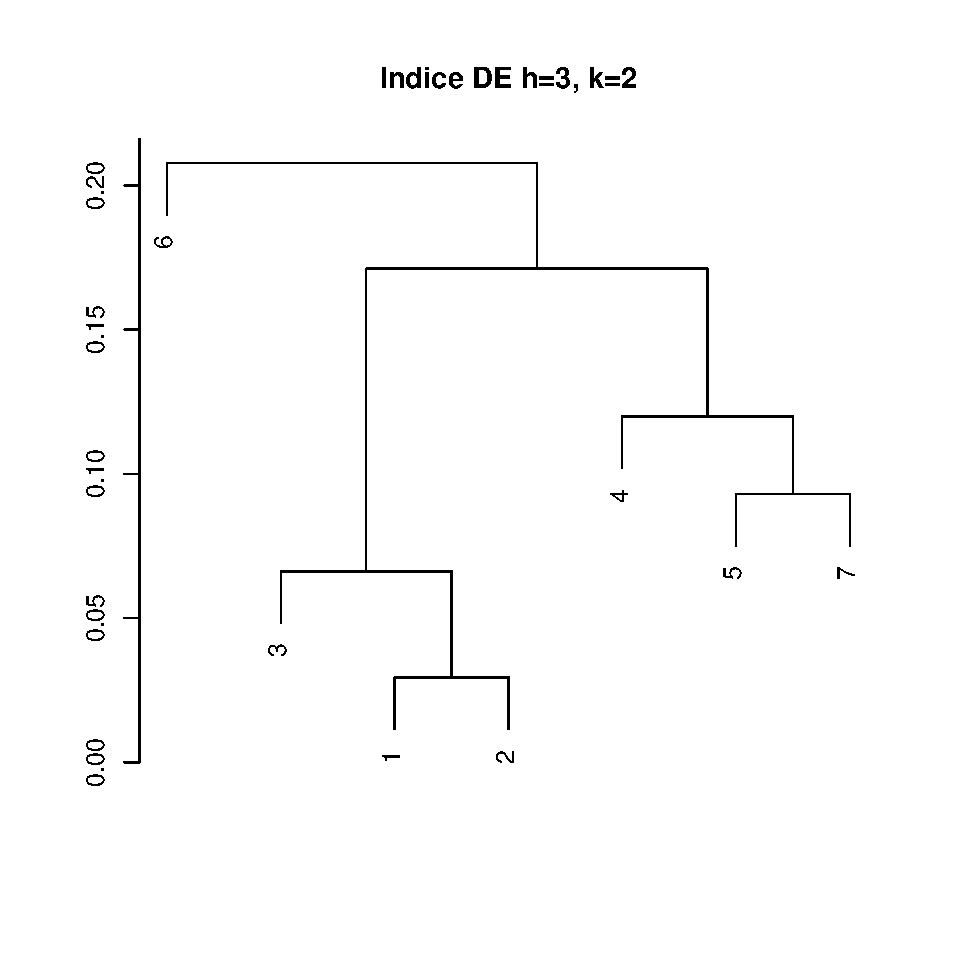
\includegraphics[height=4cm, width=4cm]{d132.eps}
       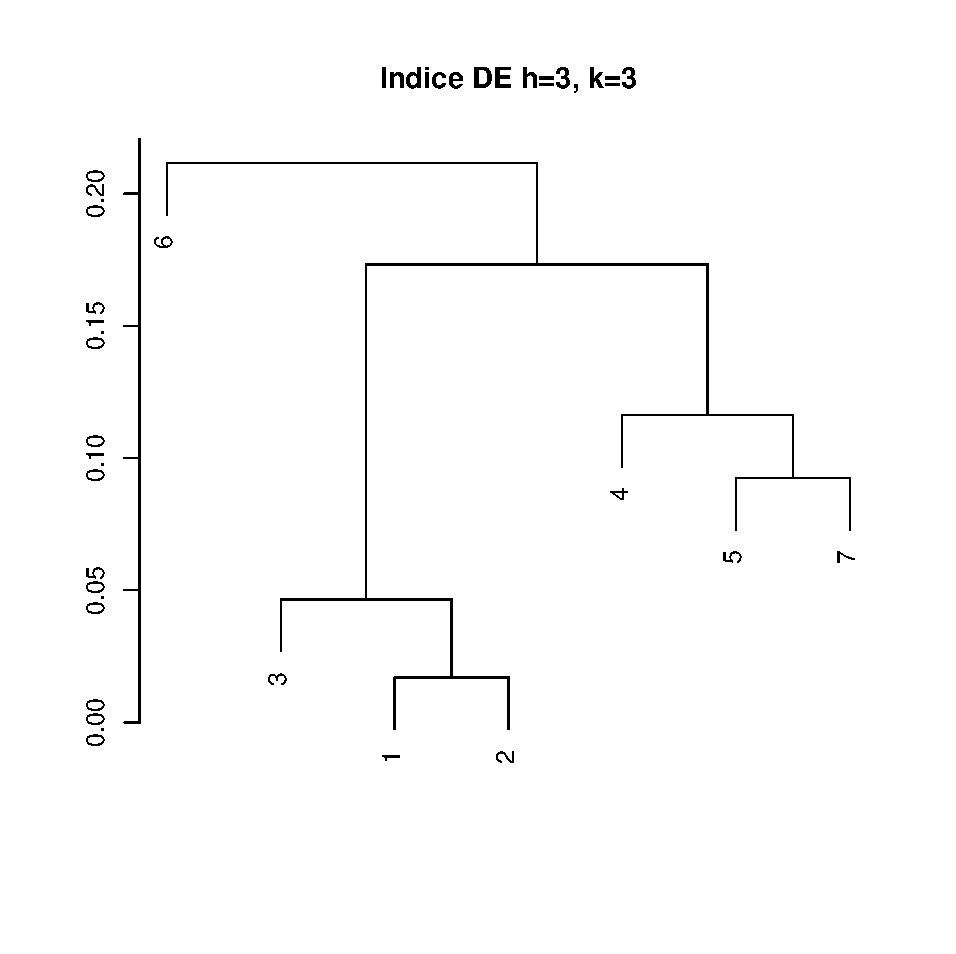
\includegraphics[height=4cm, width=4cm]{d133.eps}
       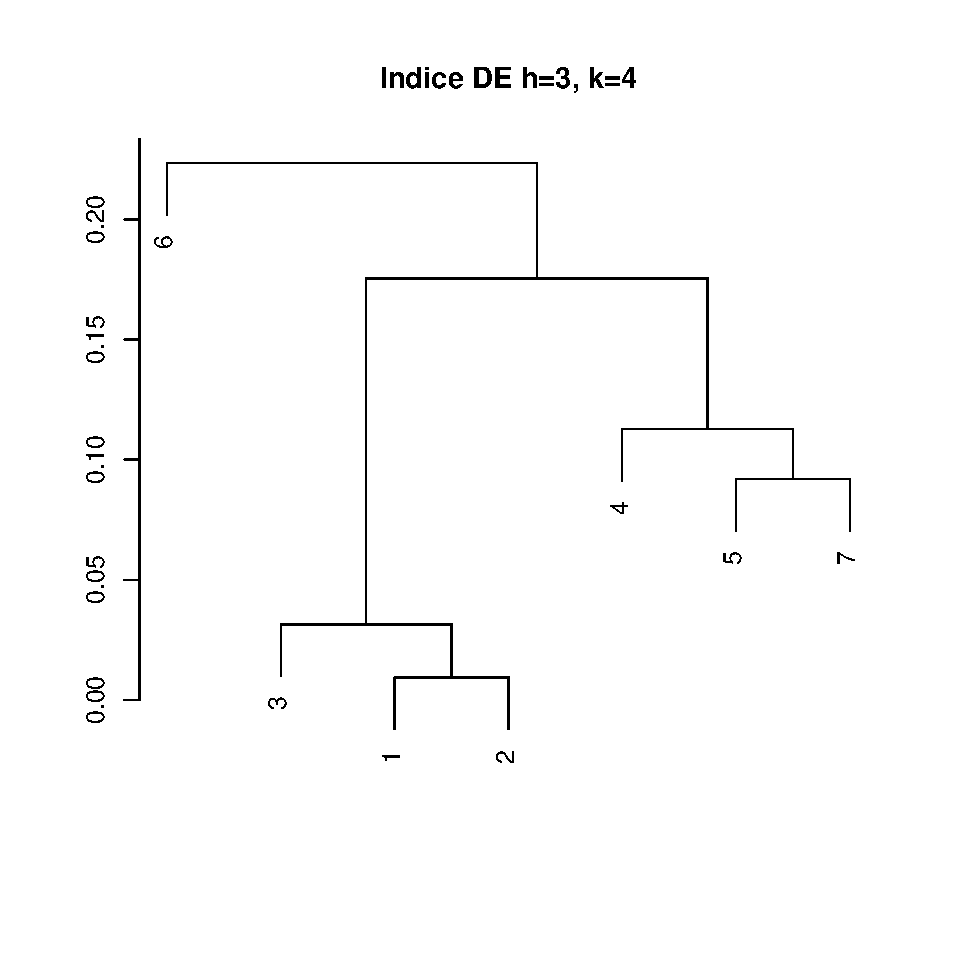
\includegraphics[height=4cm, width=4cm]{d134.eps}
\caption{Dendogramas \'Indice con $\delta_{E}$ con $h=3$, $k=1,2,3,4.$}
\label{caja}
\end{figure}


\subsection{\'Indice de Disimilaridad Adaptativo con Distancia DTW}
De igual forma que anteriormente calculamos el \'Indice de Disimilaridad Adaptativo con la Distancia  DTW con $h=1,2,3$ y $k=1,2,3,4$, se observan los siguientes resultados.

\begin{figure}[!htp]
       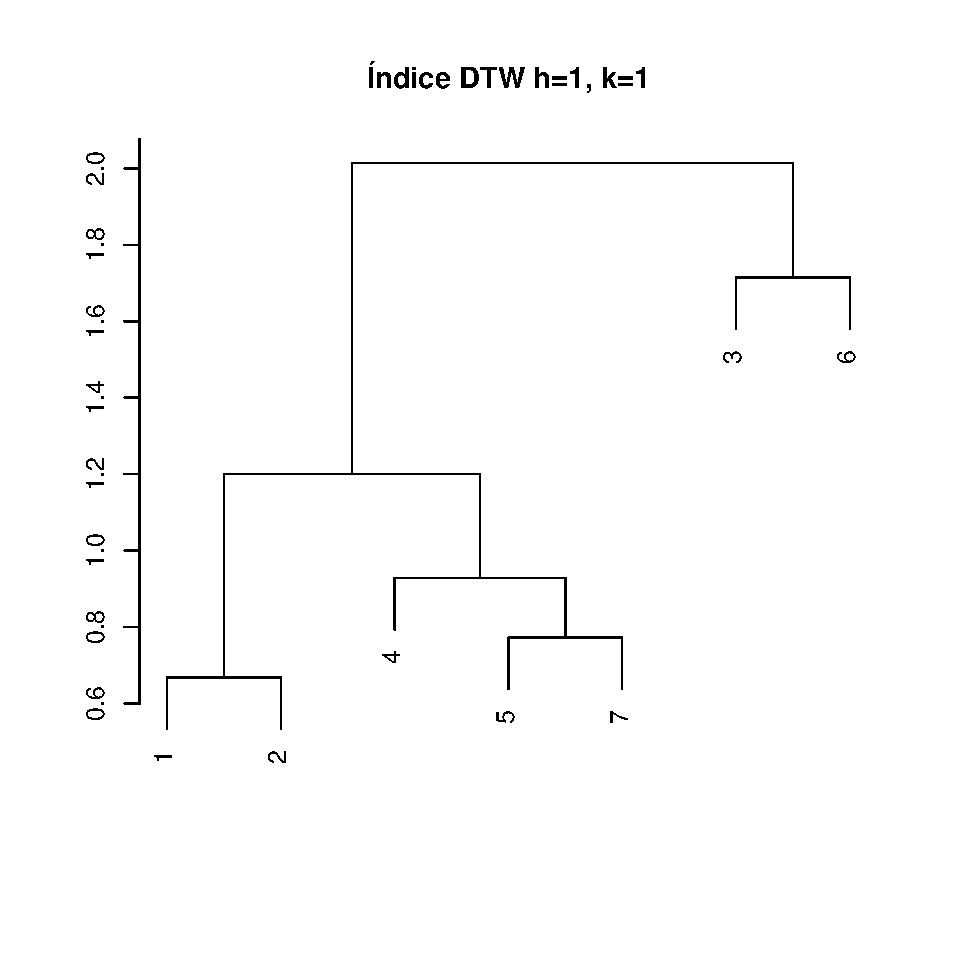
\includegraphics[height=4cm, width=4cm]{d211.eps}
       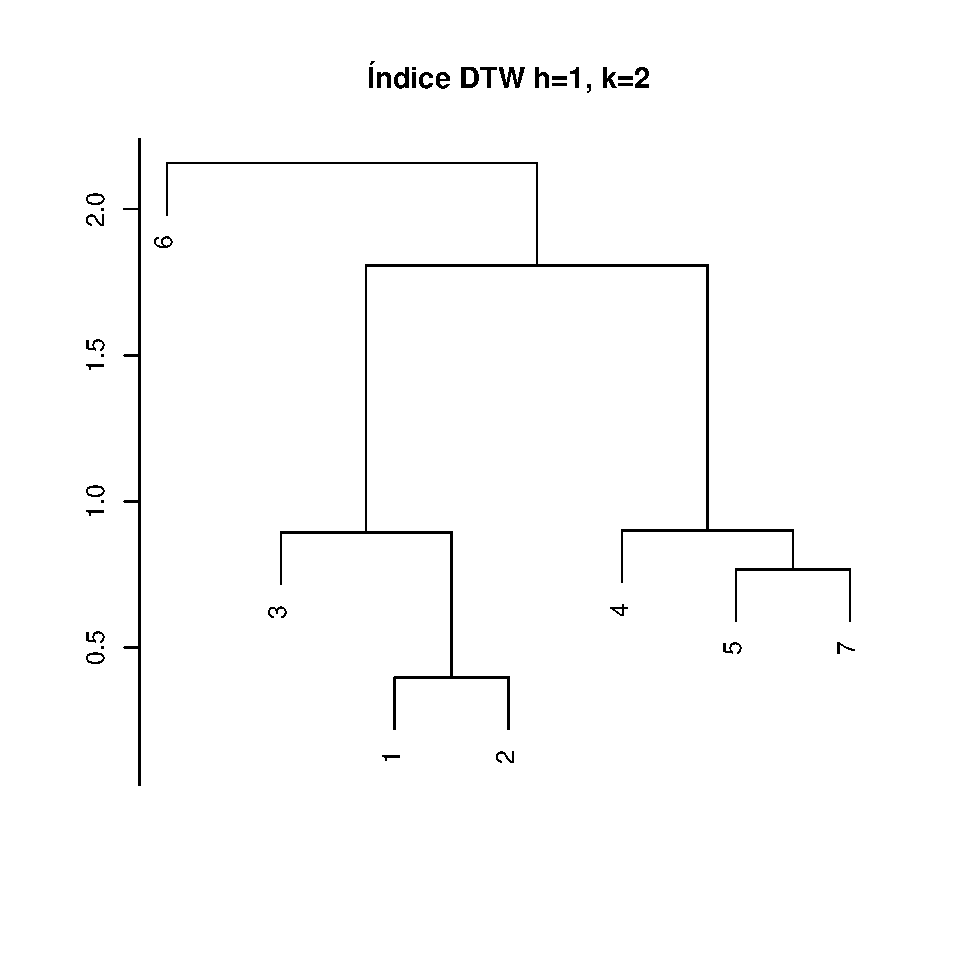
\includegraphics[height=4cm, width=4cm]{d212.eps}
       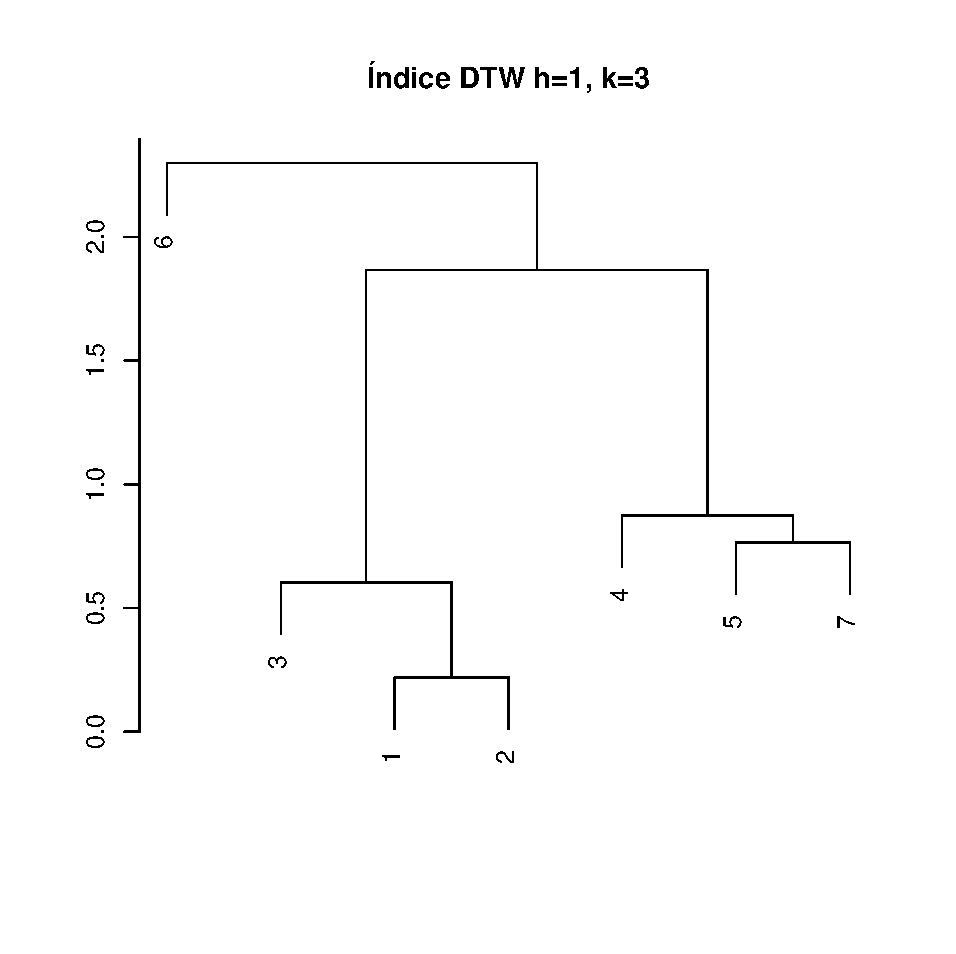
\includegraphics[height=4cm, width=4cm]{d213.eps}
       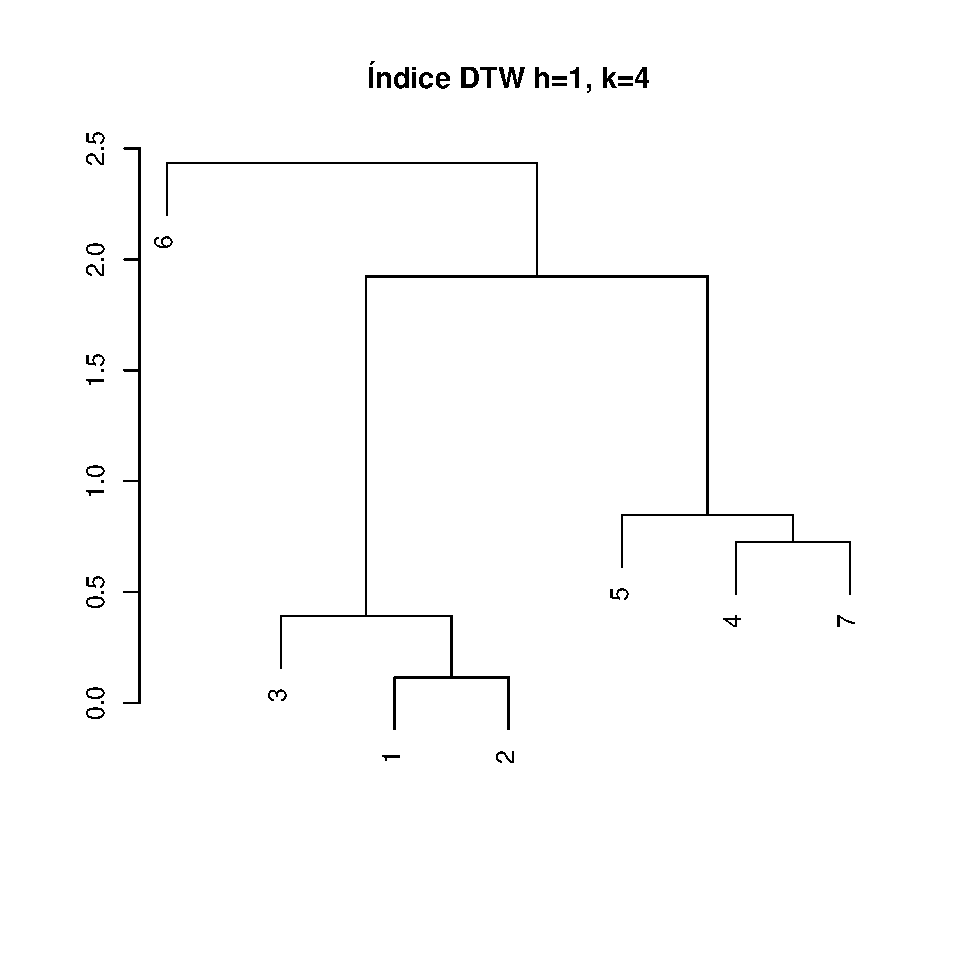
\includegraphics[height=4cm, width=4cm]{d214.eps}
\caption{Dendogramas \'Indice con $\delta_{DTW}$ con $h=1$, $k=1,2,3,4.$}
\label{caja}
\end{figure}

En el este caso con $h=1$ y $k=1$, el \'Indice no agrup\'o las series esperadas. No obstante, con $k=2,3$, el \'Indice agrupa las series esperadas.

\begin{figure}[!htp]
       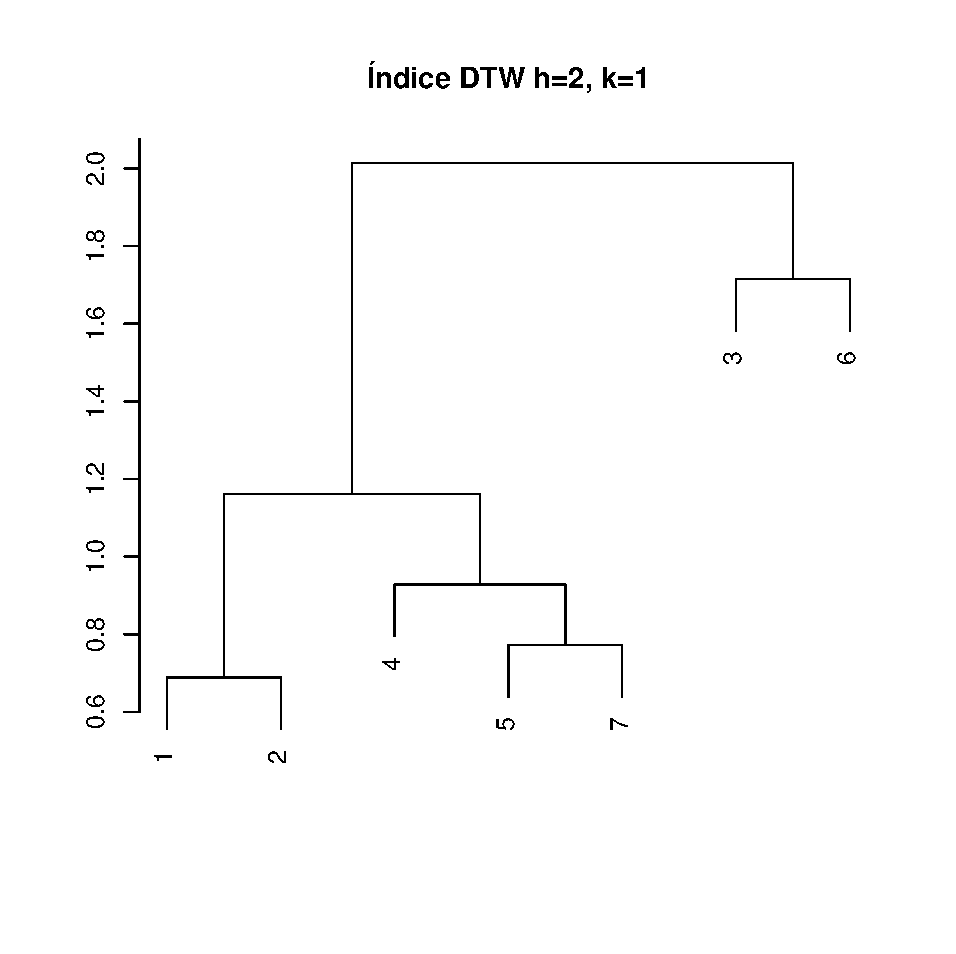
\includegraphics[height=4cm, width=4cm]{d221.eps}
       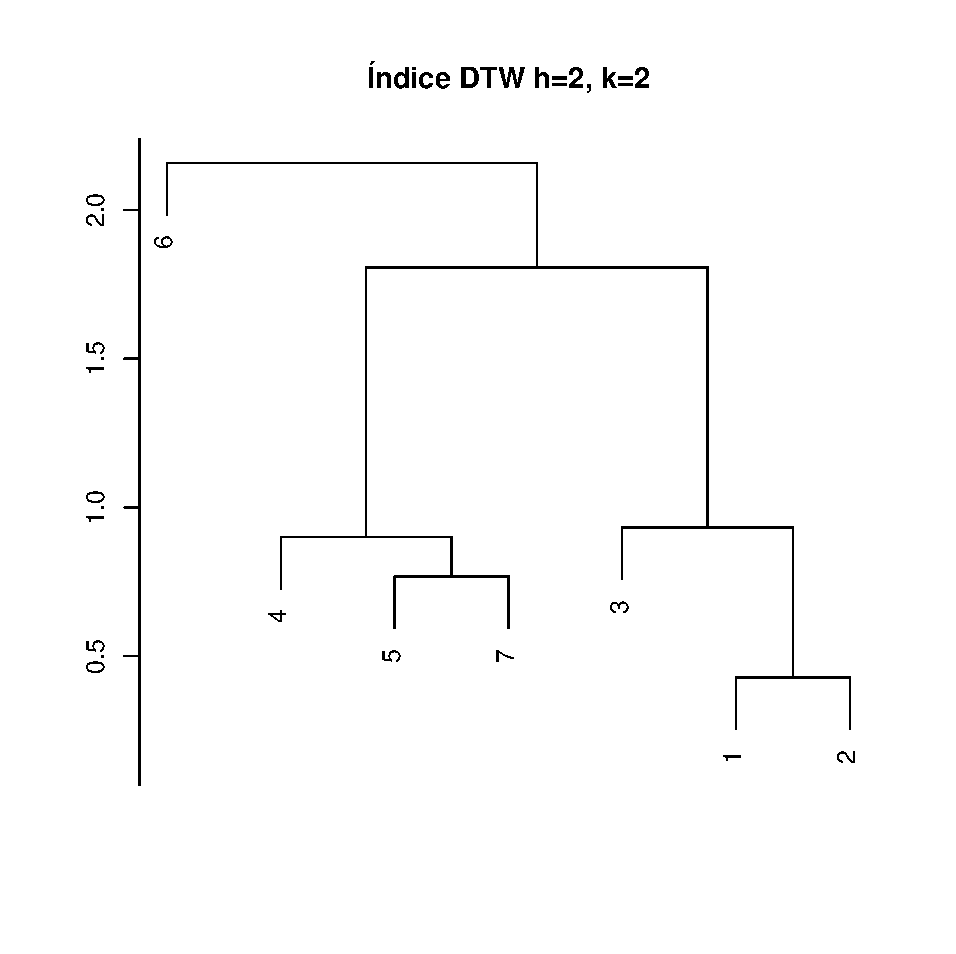
\includegraphics[height=4cm, width=4cm]{d222.eps}
       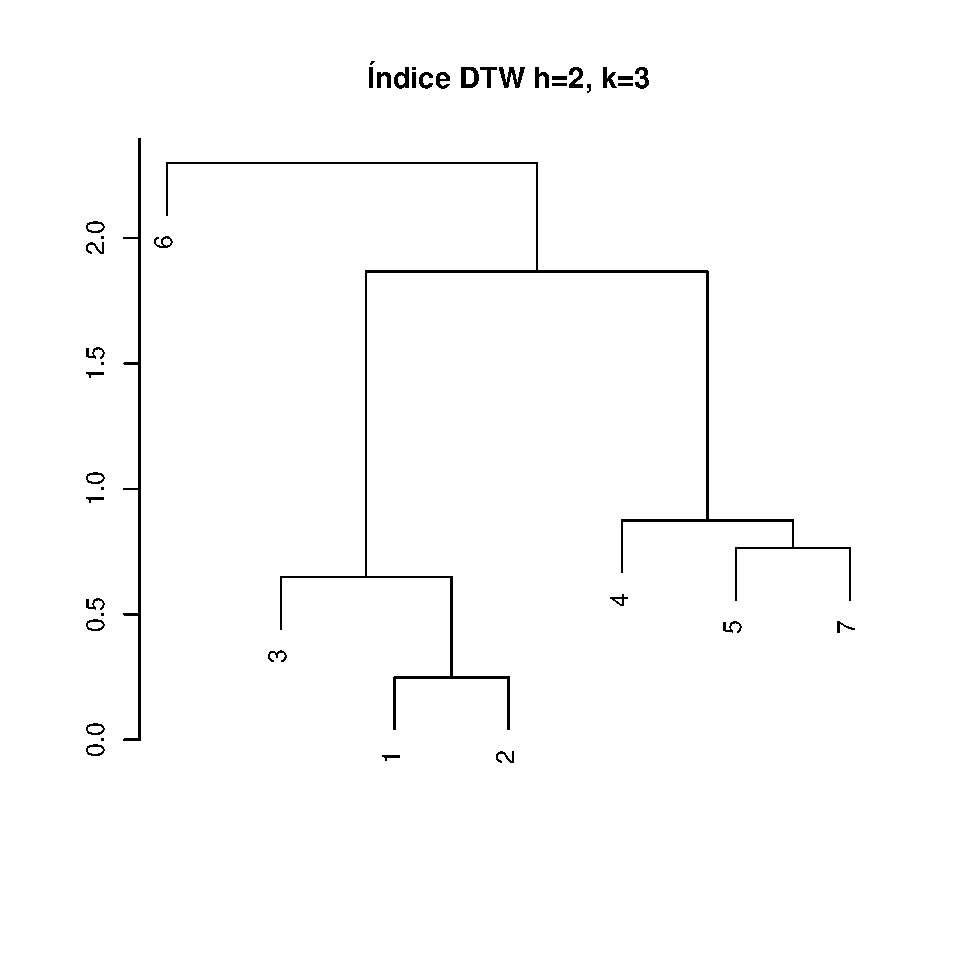
\includegraphics[height=4cm, width=4cm]{d223.eps}
       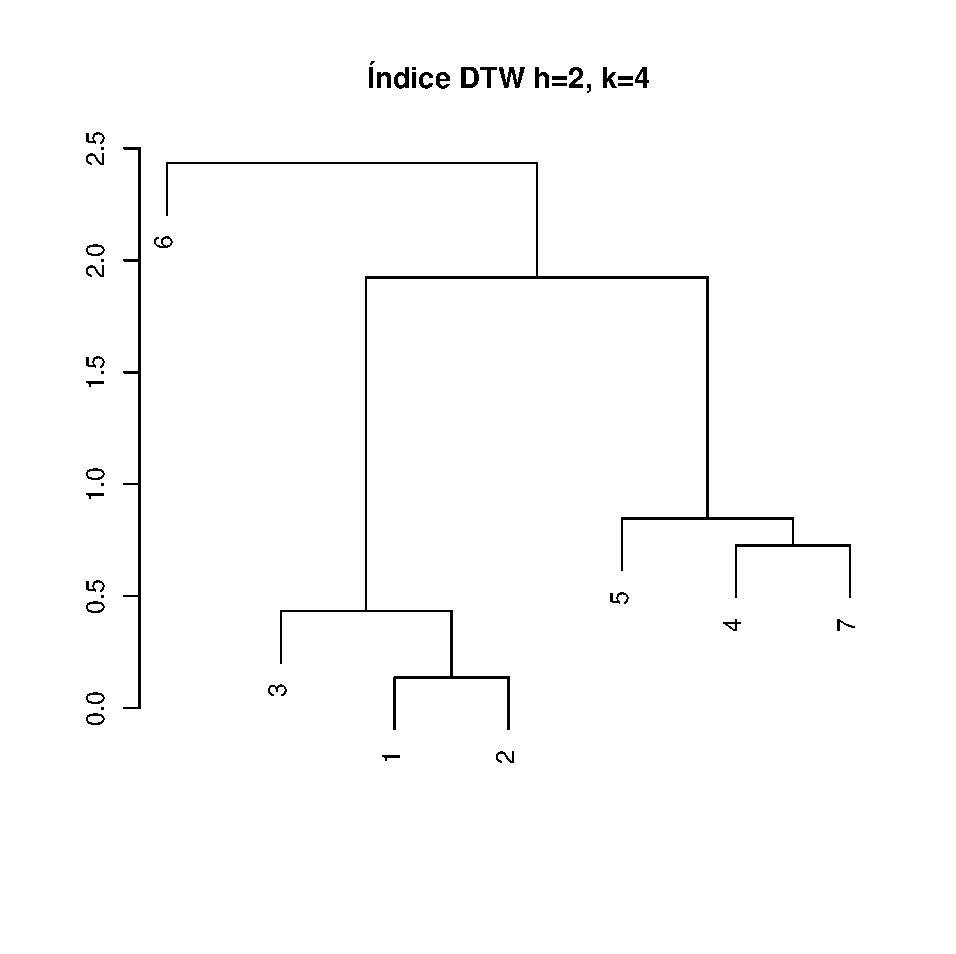
\includegraphics[height=4cm, width=4cm]{d224.eps}
\caption{Dendogramas \'Indice con $\delta_{DTW}$ con $h=2$, $k=1,2,3,4.$}
\label{caja}
\end{figure}

\begin{figure}[!htp]
       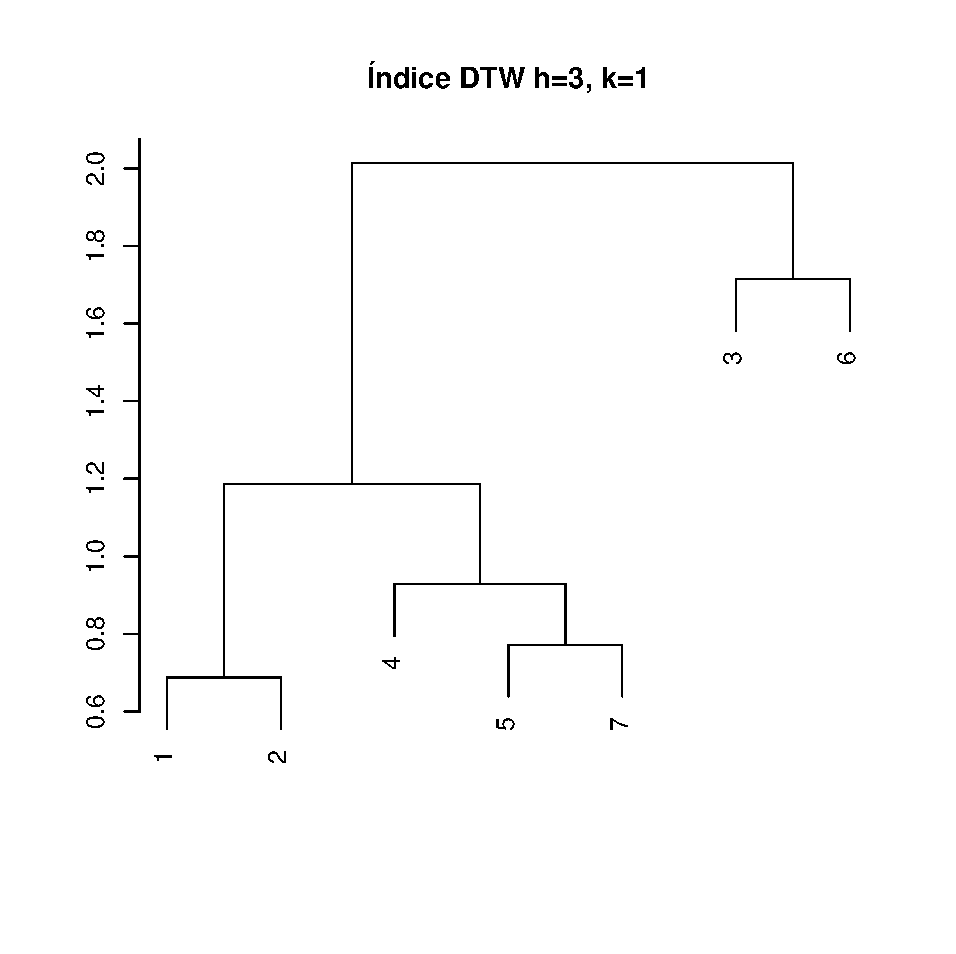
\includegraphics[height=4cm, width=4cm]{d231.eps}
       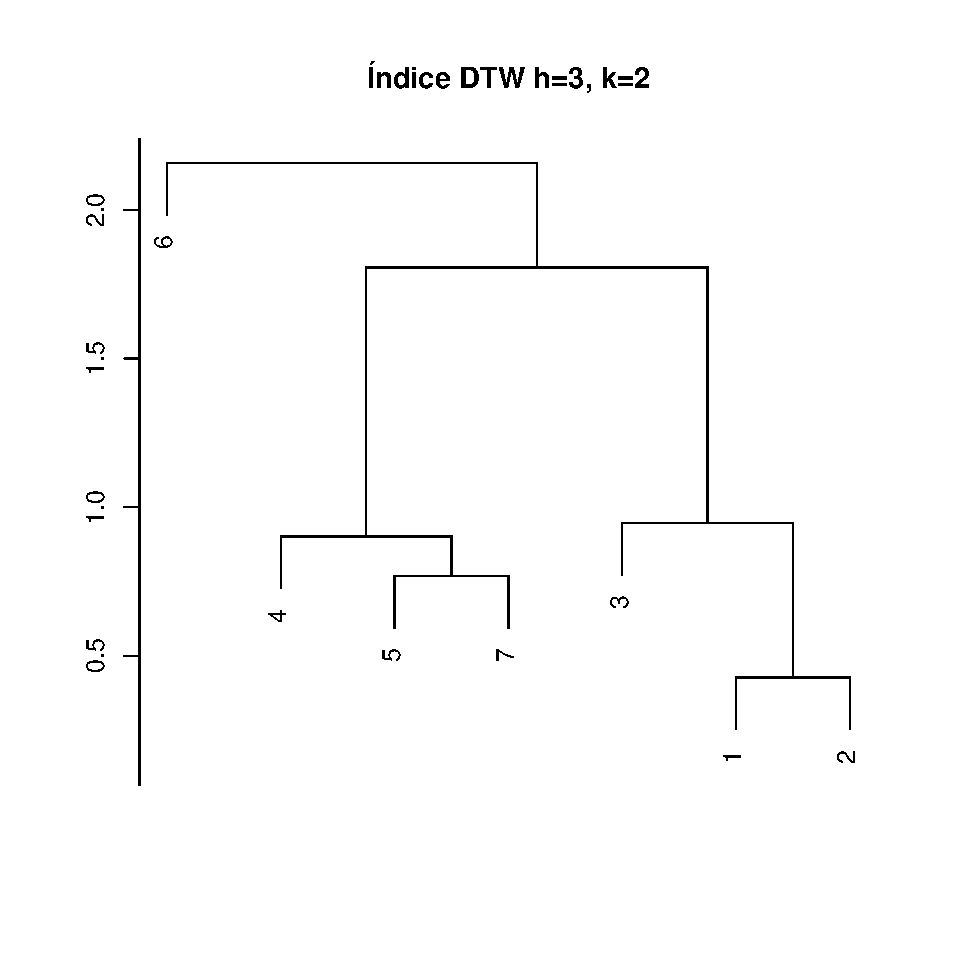
\includegraphics[height=4cm, width=4cm]{d232.eps}
       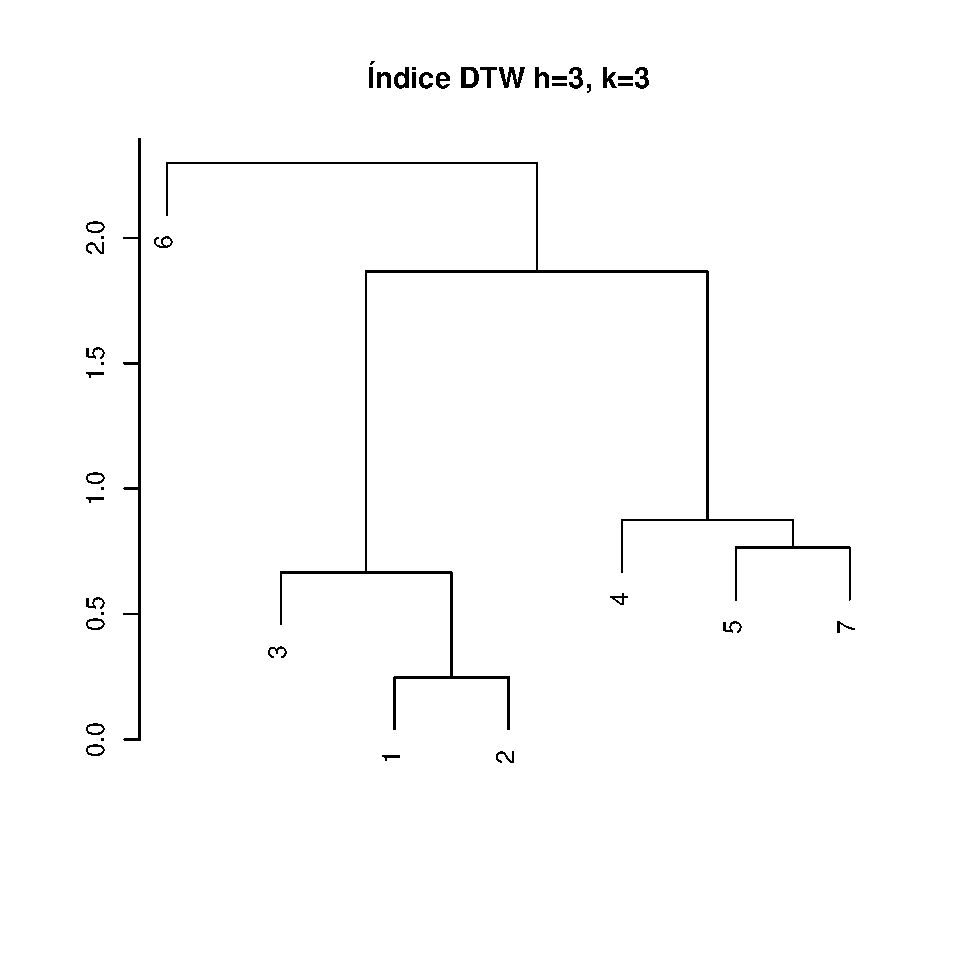
\includegraphics[height=4cm, width=4cm]{d233.eps}
       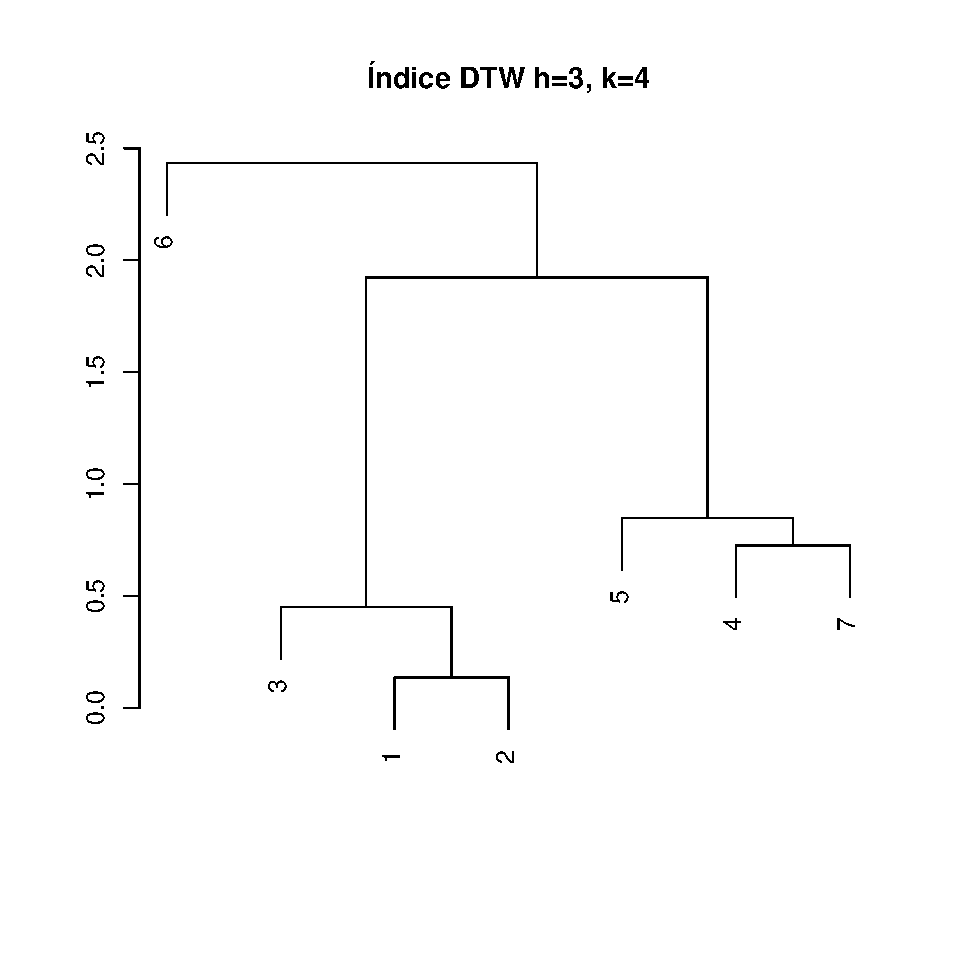
\includegraphics[height=4cm, width=4cm]{d234.eps}
\caption{Dendogramas \'Indice con $\delta_{DTW}$ con $h=3$, $k=1,2,3,4.$}
\label{caja}
\end{figure}

De igual manera sucede con $h=2$ y $k=1$ el algoritmo clasifica dos de las tres series. Con $h=2$, $h=3$ y $k=2,3$ el algoritmo vuelve agrupar las series se simularon.

\subsection{\'Indice de Disimilaridad Adaptativo con Distancia de Frech\'et}
Finalmente si se calcula el \'Indice de Disimilaridad con Distancia se Frech\'et, se pueden observar los siguientes resultados. El \'Indice calculado con $h=1,2$ y $k=1,2,3$ muestra algunas variaciones con los resultados esperados, ya que, el \'indice no logra percibir las diferencias entre las correlaciones. Por otra parte, con $h=3$ y  $k=1$, el \'Indice agrupa las series $X_t$, $Y_t$ y $W_t$.\\
De igual forma se puede apreciar que el \'Indice va agrupar mejor con altos valores de $h$ y $k$.


\begin{figure}[!htp]
       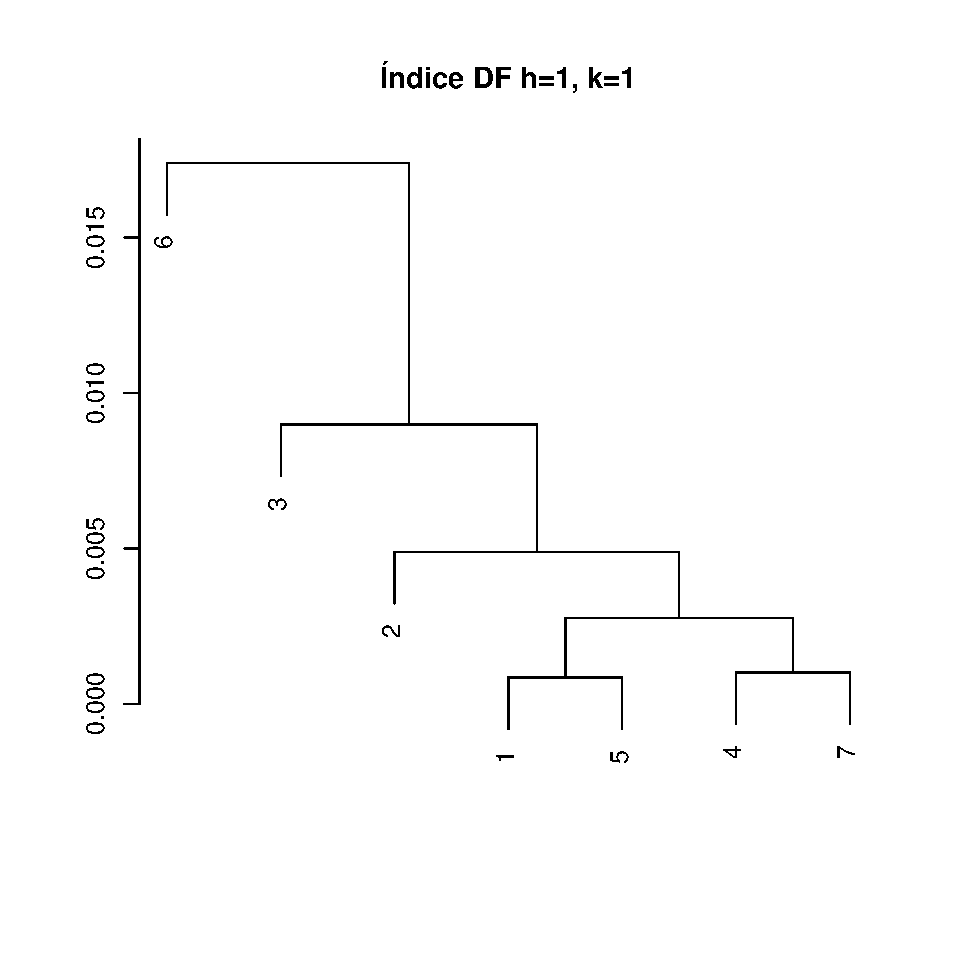
\includegraphics[height=4cm, width=4cm]{d311.eps}
       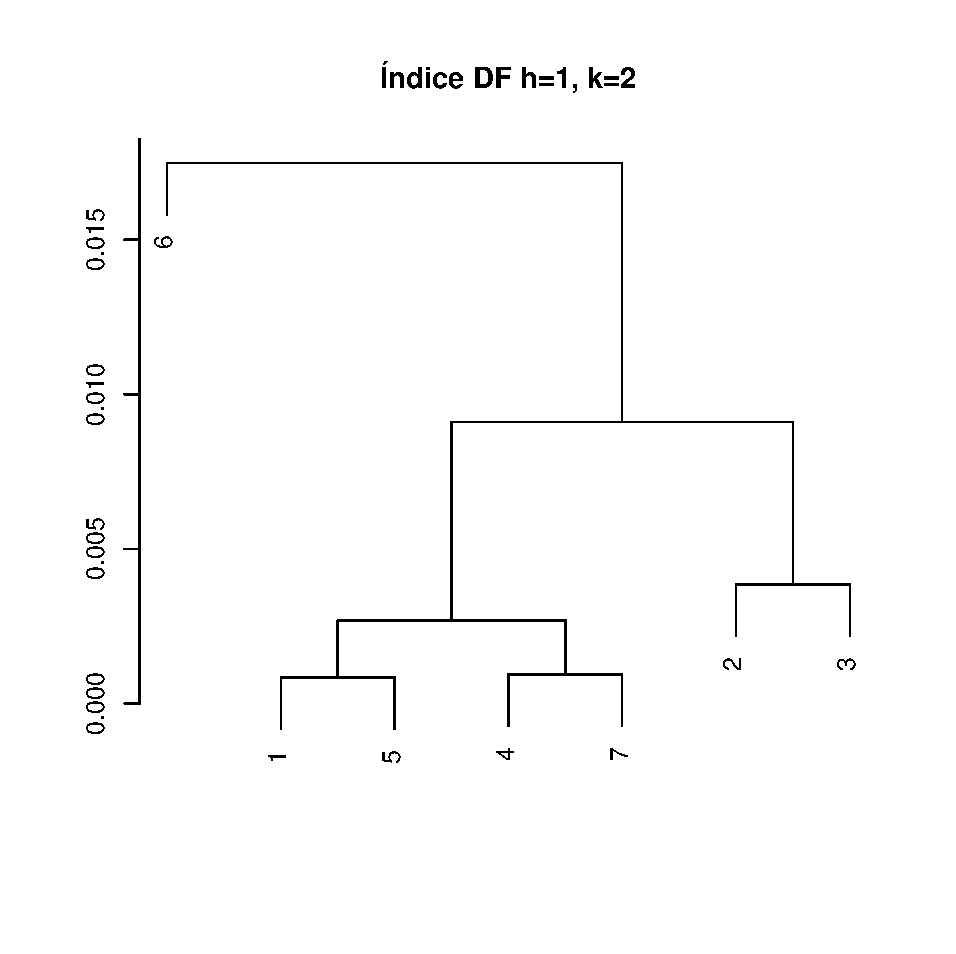
\includegraphics[height=4cm, width=4cm]{d312.eps}
       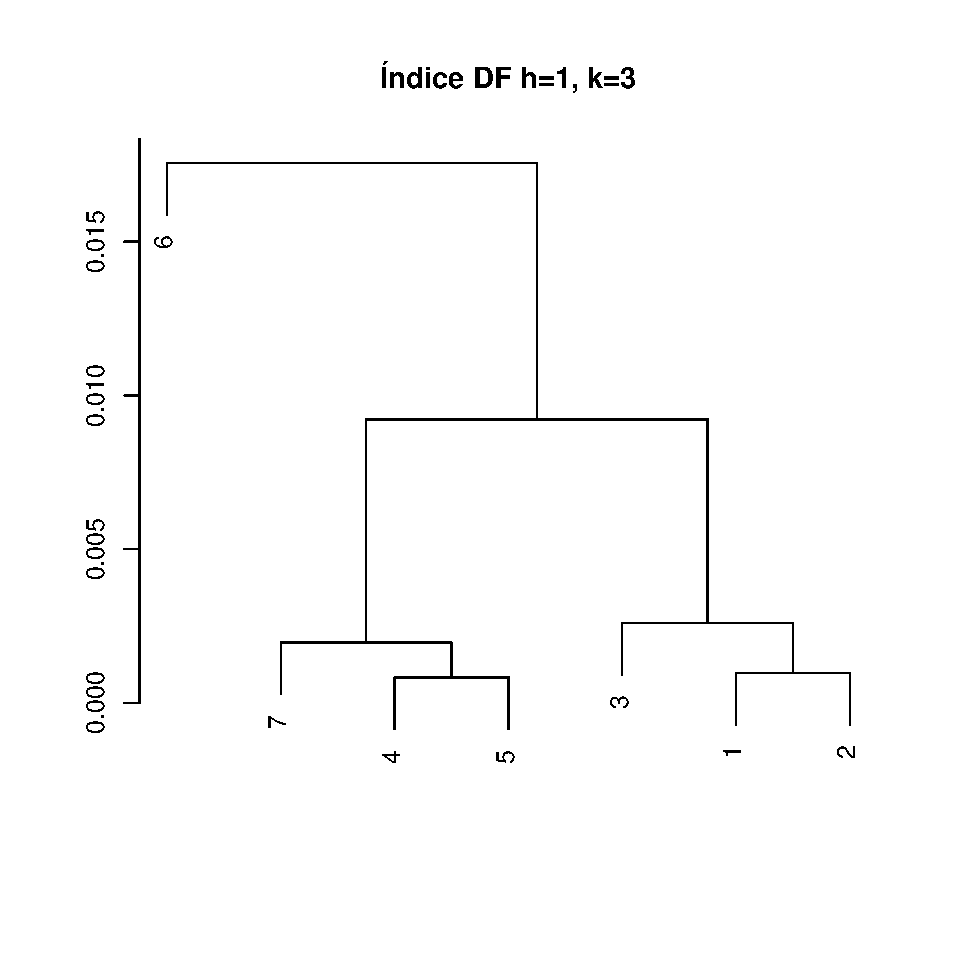
\includegraphics[height=4cm, width=4cm]{d313.eps}
       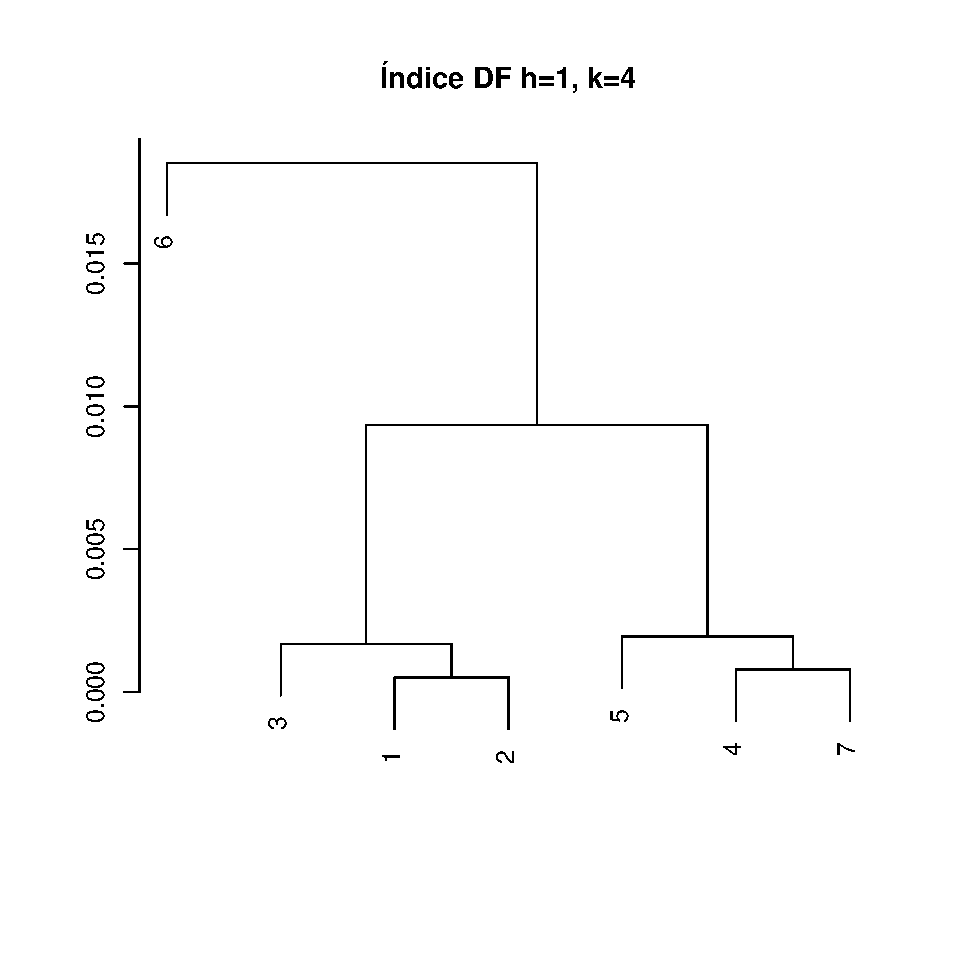
\includegraphics[height=4cm, width=4cm]{d314.eps}
\caption{Dendogramas \'Indice con $\delta_{F}$ con $h=1$, $k=1,2,3,4.$}
\label{caja}
\end{figure}


\begin{figure}[!htp]
       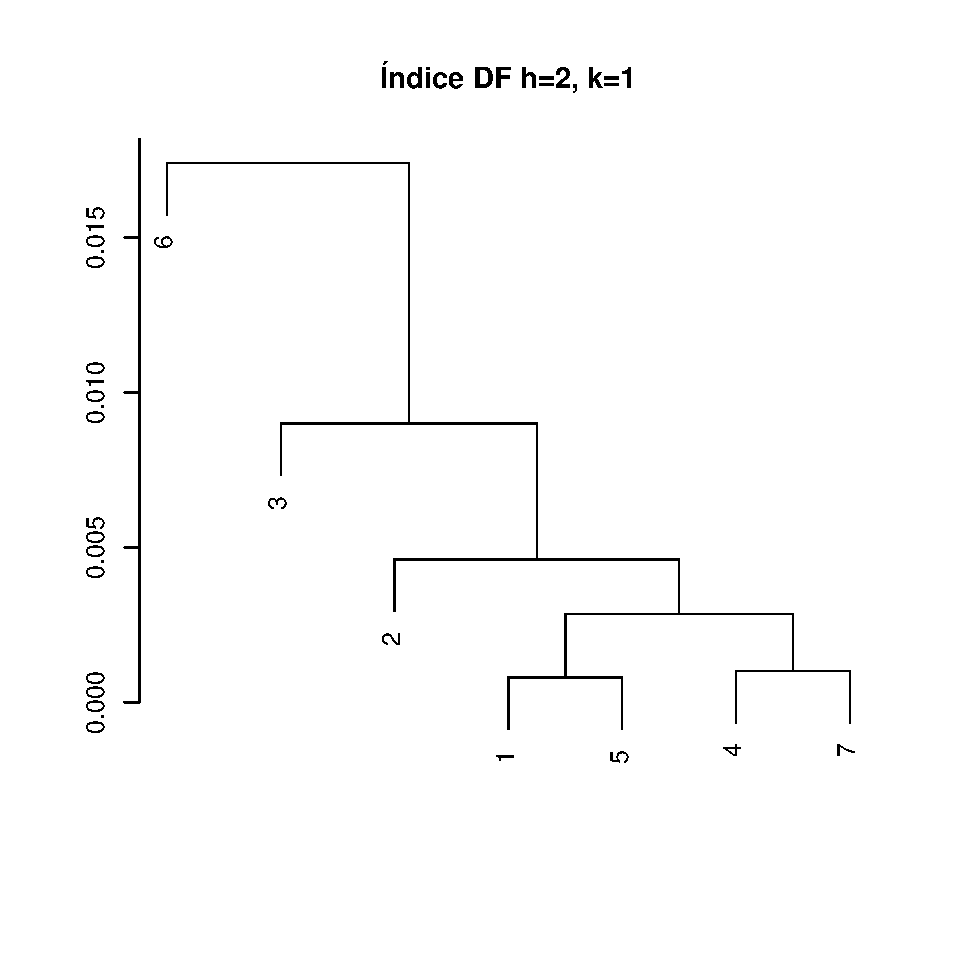
\includegraphics[height=4cm, width=4cm]{d321.eps}
       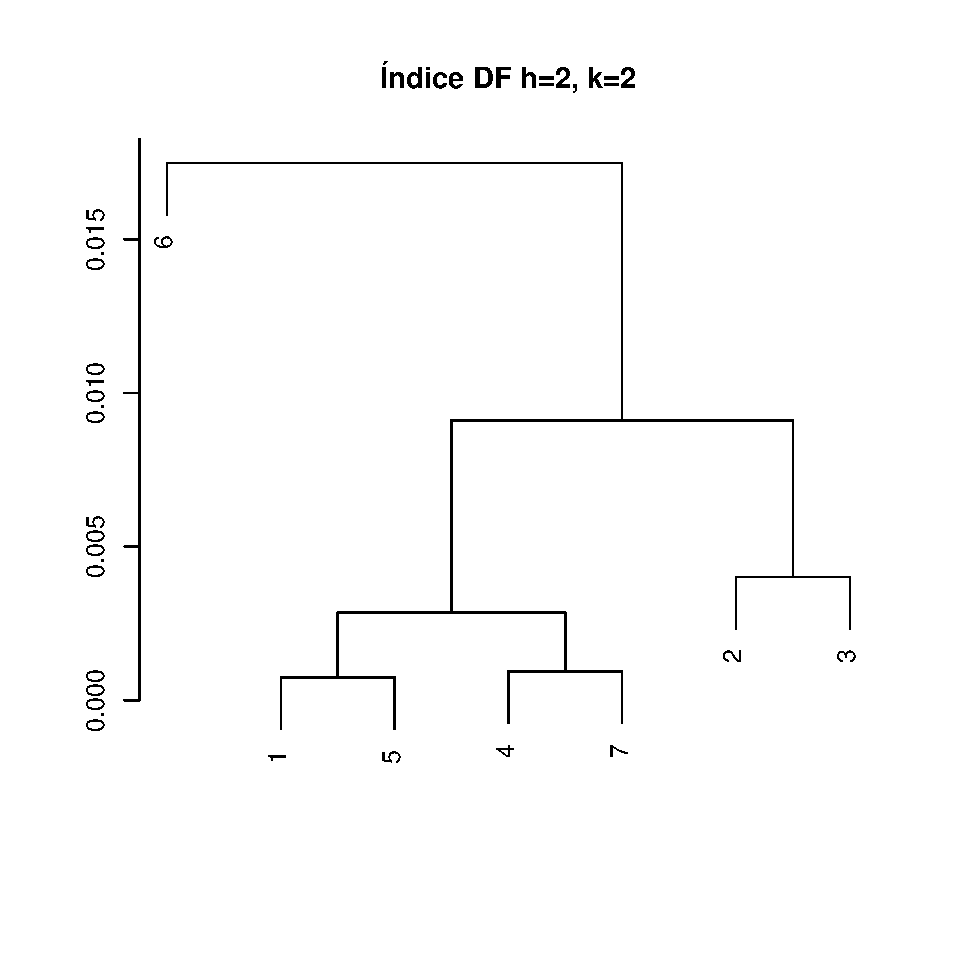
\includegraphics[height=4cm, width=4cm]{d322.eps}
       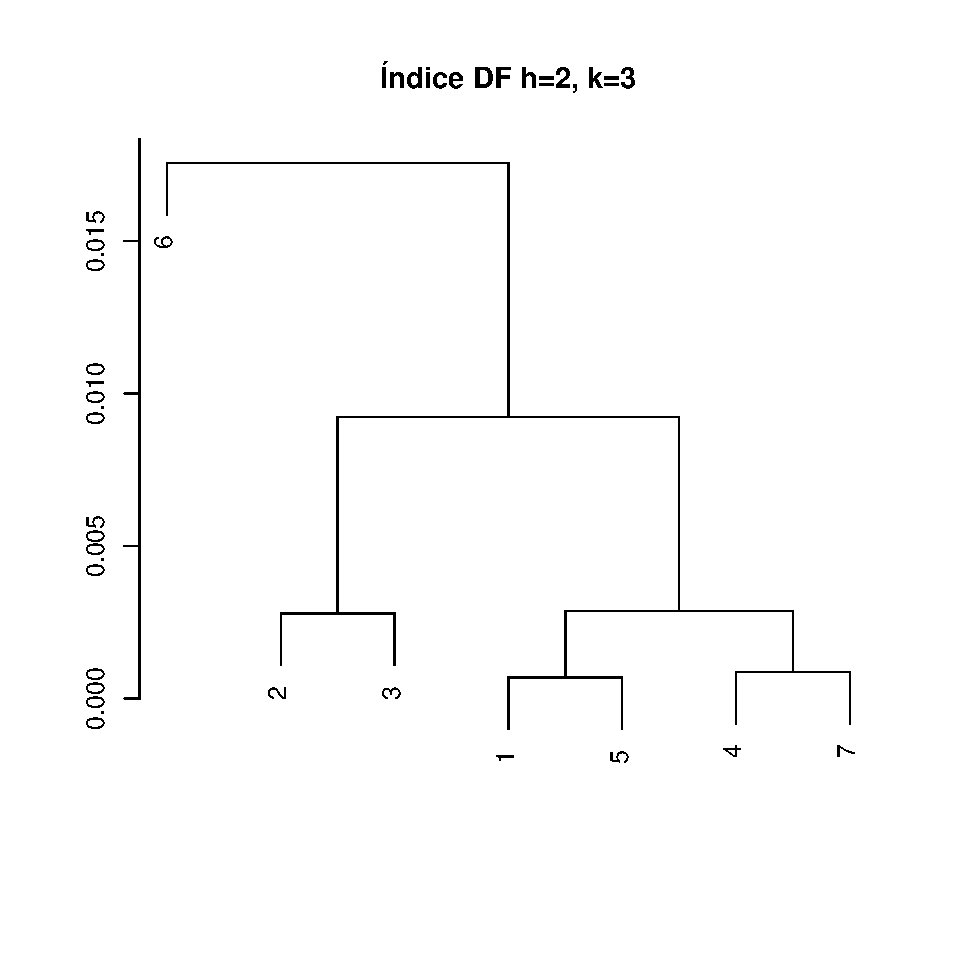
\includegraphics[height=4cm, width=4cm]{d323.eps}
       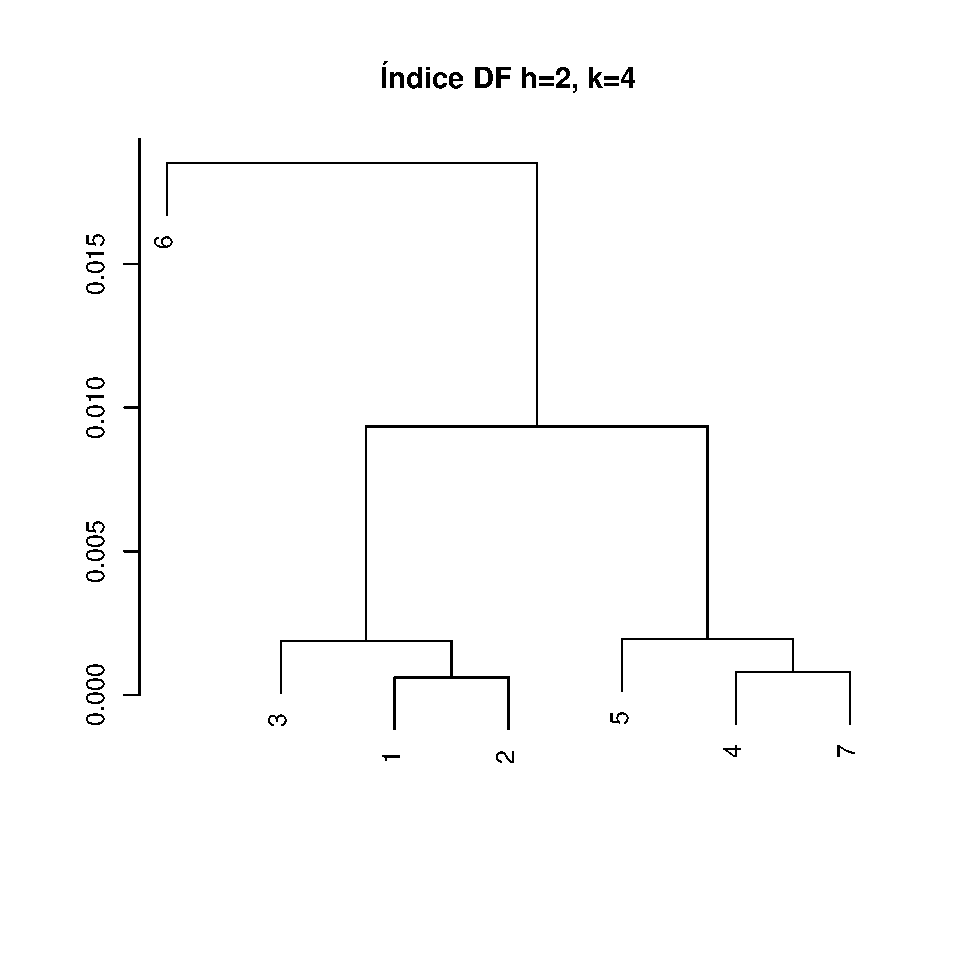
\includegraphics[height=4cm, width=4cm]{d324.eps}
\caption{Dendogramas \'Indice con $\delta_{F}$ con $h=2$, $k=1,2,3,4.$}
\label{caja}
\end{figure}

\begin{figure}[!htp]
       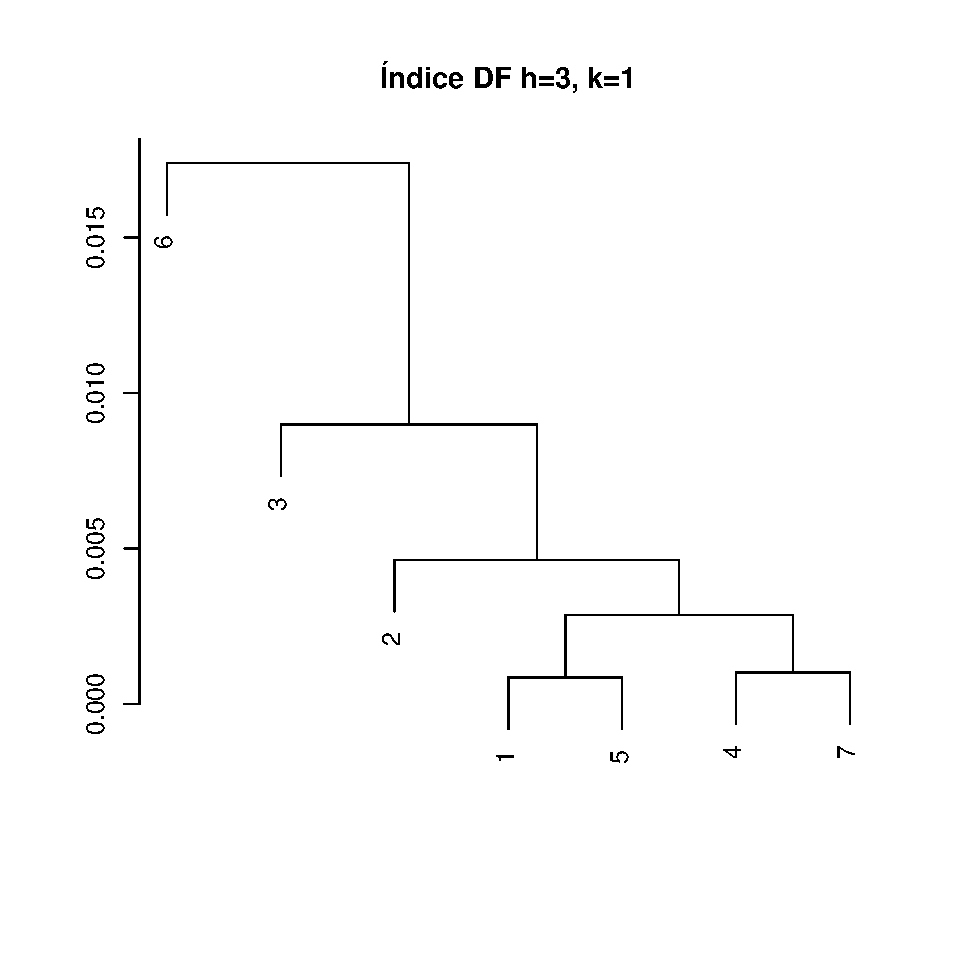
\includegraphics[height=4cm, width=4cm]{d331.eps}
       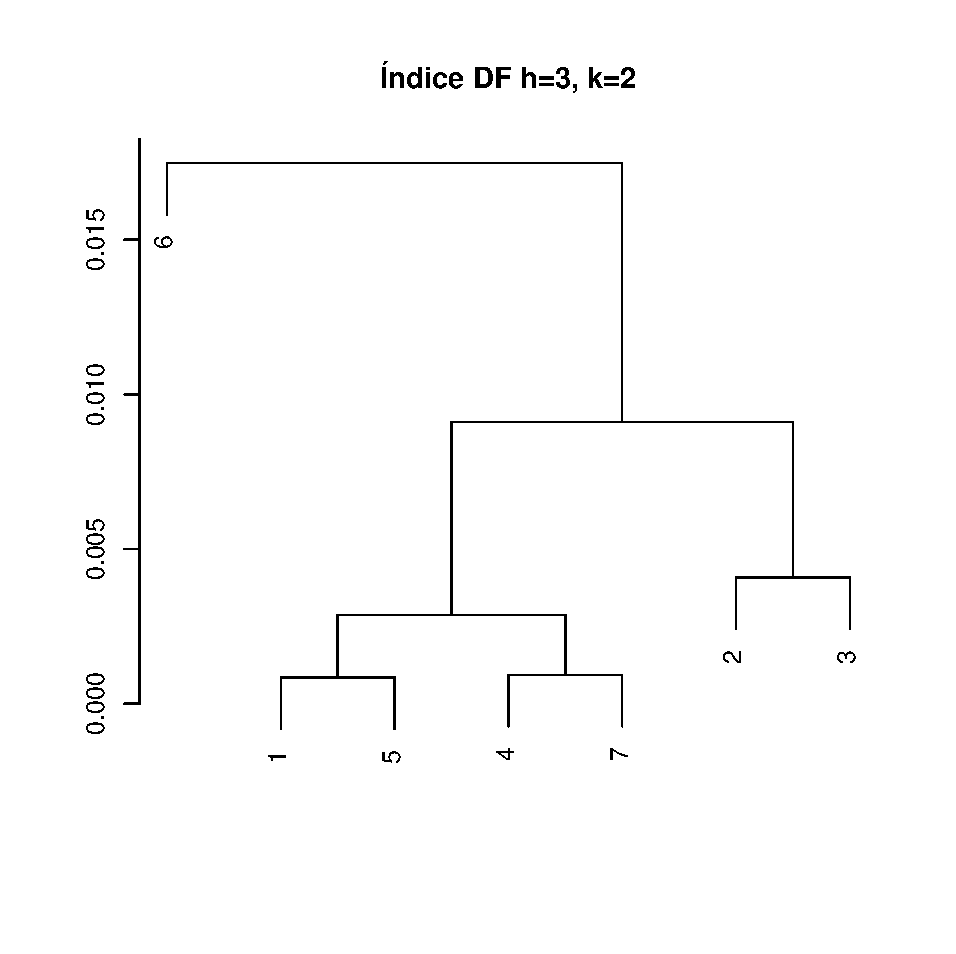
\includegraphics[height=4cm, width=4cm]{d332.eps}
       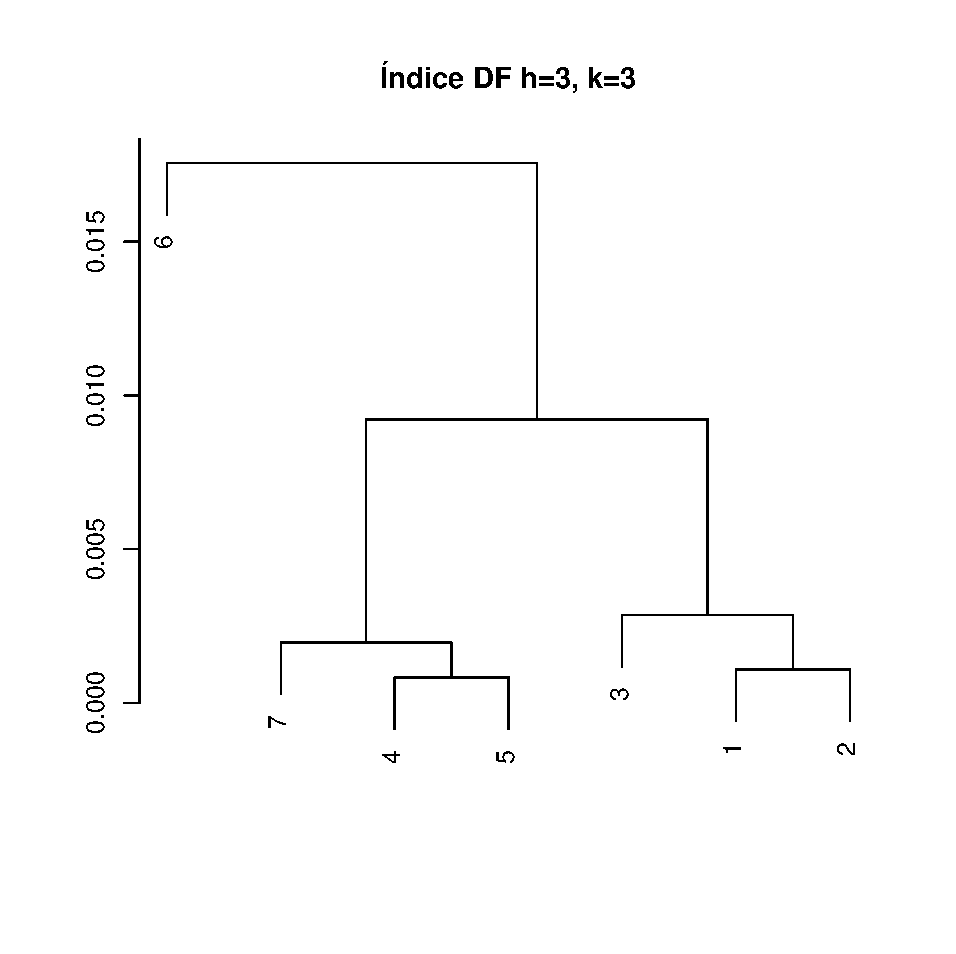
\includegraphics[height=4cm, width=4cm]{d333.eps}
       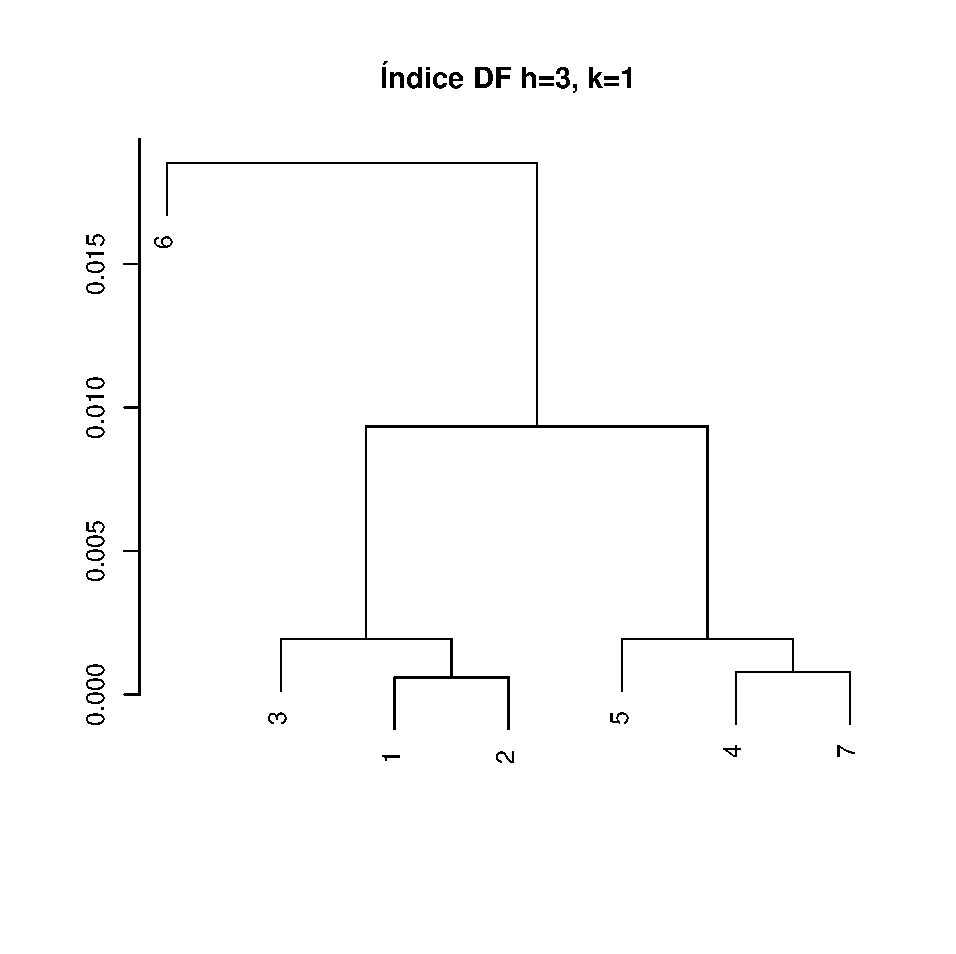
\includegraphics[height=4cm, width=4cm]{d334.eps}
\caption{Dendogramas \'Indice con $\delta_{F}$ con $h=3$, $k=1,2,3,4.$}
\label{caja}
\end{figure}

\newpage

\section{Conclusi\'on}
En los dendogramas se puede apreciar que el \'Indice de Disimilaridad con distancia euclidiana y DTW agrupa las series correlacionadas.

El \'Indice con la distancia de Frech\'et presenta una variaci\'on en la agrupaci\'on, ya que para valores altos de $h$ y $k$, los resultados son alcanzados.

La funci\'on de $k$, en el \'Indice de Disimilaridad modula la contribuci\'on del comovimiento respecto del comportamiento de los valores respecto a su cercan\'ia, esto se puede apreciar mejor cuando las distancias son poco sensibles, ya que para valores altos de $k$, la distancia convencional se ve afectada por una mayor contribuci\'on al comportamiento respecto del comovimiento, es decir, para valores de $k\geq 3$ la distancia convencional sera mas sensible a los cambios del comportamiento respecto de su comovimiento.

Es importante, calcular el \'Indice con distintos valores de h y k, para verificar y sacar conclusiones respecto de los grupos establecidos por esta nueva medida.

La simulaci\'on a demostrado que el \'Indice de Disimilaridad agrupa series temporales considerando su estructura de comovimiento y el comportamiento a su cercan\'ia, es decir, el \'Indice agrupa las series que est\'an fuertemente correlacionadas.

Se demostr\'o que las medidas convencionales ignoran la relaci\'on de interdependencia entre las medidas, ya que, son primordialmente basadas en la proximidad con relaci\'on a los valores.

%\section{Comparaci\'on de coeficientes anteriores para modelos ARMA.}

%\section{Compararci\'on de $D({X_{t}},{Y_{t}})$ con diferentes funciones.}


%\section{An\'alisis de la estacionalidad.}
%Por definir
%\section{Robustez de los coeficientes.}

% ------------------------------------------------------------------------
